%%%%%%%%%%%%%%%%%%%%%%%%%%%%%%%%%%%%%%%%%%%%%%%%%%%%%%%%%%%%%%%%%%%%%%%%%%%%
% AGUJournalTemplate.tex: this template file is for articles formatted with LaTeX
%
% This file includes commands and instructions
% given in the order necessary to produce a final output that will
% satisfy AGU requirements, including customized APA reference formatting.
%
% You may copy this file and give it your
% article name, and enter your text.
%
%
% Step 1: Set the \documentclass
%
%

%% To submit your paper:
\documentclass[draft]{agujournal2019}
\usepackage{url} %this package should fix any errors with URLs in refs.
\usepackage{lineno}
\usepackage[inline]{trackchanges} %for better track changes. finalnew option will compile document with changes incorporated.
\usepackage{soul}
\usepackage{amsmath}
\usepackage{siunitx}
\usepackage{color}
\newcommand{\red}[1]{\textcolor{red}{#1}}
\newcommand{\blue}[1]{\textcolor{blue}{#1}}
\newcommand{\rout}[1]{\red{\sout{#1}}}
\newcommand{\ab}[1]{\textcolor{Blue}{\sout{#1}}}

\linenumbers
%%%%%%%
% As of 2018 we recommend use of the TrackChanges package to mark revisions.
% The trackchanges package adds five new LaTeX commands:
%
%  \note[editor]{The note}
%  \annote[editor]{Text to annotate}{The note}
%  \add[editor]{Text to add}
%  \remove[editor]{Text to remove}
%  \change[editor]{Text to remove}{Text to add}
%
% complete documentation is here: http://trackchanges.sourceforge.net/
%%%%%%%

\draftfalse

%% Enter journal name below.
%% Choose from this list of Journals:
%
% JGR: Atmospheres
% JGR: Biogeosciences
% JGR: Earth Surface
% JGR: Oceans
% JGR: Planets
% JGR: Solid Earth
% JGR: Space Physics
% Global Biogeochemical Cycles
% Geophysical Research Letters
% Paleoceanography and Paleoclimatology
% Radio Science
% Reviews of Geophysics
% Tectonics
% Space Weather
% Water Resources Research
% Geochemistry, Geophysics, Geosystems
% Journal of Advances in Modeling Earth Systems (JAMES)
% Earth's Future
% Earth and Space Science
% Geohealth
%
% ie, \journalname{Water Resources Research}

\journalname{JGR: Oceans}


\begin{document}

%% ------------------------------------------------------------------------ %%
%  Title
%
% (A title should be specific, informative, and brief. Use
% abbreviations only if they are defined in the abstract. Titles that
% start with general keywords then specific terms are optimized in
% searches)
%
%% ------------------------------------------------------------------------ %%



\title{Melt Response to Calving Events in Pine Island Glacier}

%% ------------------------------------------------------------------------ %%
%
%  AUTHORS AND AFFILIATIONS
%
%% ------------------------------------------------------------------------ %%

% Authors are individuals who have significantly contributed to the
% research and preparation of the article. Group authors are allowed, if
% each author in the group is separately identified in an appendix.)

% List authors by first name or initial followed by last name and
% separated by commas. Use \affil{} to number affiliations, and
% \thanks{} for author notes.
% Additional author notes should be indicated with \thanks{} (for
% example, for current addresses).

% Example: \authors{A. B. Author\affil{1}\thanks{Current address, Antartica}, B. C. Author\affil{2,3}, and D. E.
% Author\affil{3,4}\thanks{Also funded by Monsanto.}}

\authors{A. T. Bradley\affil{1}, D. Bett\affil{1}, P. Dutrieux\affil{1}, J. De Rydt\affil{2}, P. R Holland\affil{1}}


% \affiliation{1}{First Affiliation}
% \affiliation{2}{Second Affiliation}
% \affiliation{3}{Third Affiliation}
% \affiliation{4}{Fourth Affiliation}

\affiliation{1}{British Antarctic Survey, High Cross, Madingley Road, Cambridge CB3 0ET, UK}
\affiliation{2}{Department of Geography and Environmental Sciences, Northumbria University, Newcastle upon Tyne, UK.}

%(repeat as many times as is necessary)

%% Corresponding Author:
% Corresponding author mailing address and e-mail address:

% (include name and email addresses of the corresponding author.  More
% than one corresponding author is allowed in this LaTeX file and for
% publication; but only one corresponding author is allowed in our
% editorial system.)

% Example: \correspondingauthor{First and Last Name}{email@address.edu}

\correspondingauthor{Alexander Bradley}{aleey@bas.ac.uk}

%% Keypoints, final entry on title page.

%  List up to three key points (at least one is required)
%  Key Points summarize the main points and conclusions of the article
%  Each must be 100 characters or less with no special characters or punctuation and must be complete sentences

% Example:
% \begin{keypoints}
% \item	List up to three key points (at least one is required)
% \item	Key Points summarize the main points and conclusions of the article
% \item	Each must be 100 characters or less with no special characters or punctuation and must be complete sentences
% \end{keypoints}

%\begin{keypoints}
%\item 
%\item
%\item  
%\end{keypoints}

%% ------------------------------------------------------------------------ %%
%
%  ABSTRACT and PLAIN LANGUAGE SUMMARY
%
% A good Abstract will begin with a short description of the problem
% being addressed, briefly describe the new data or analyses, then
% briefly states the main conclusion(s) and how they are supported and
% uncertainties.

% The Plain Language Summary should be written for a broad audience,
% including journalists and the science-interested public, that will not have 
% a background in your field.
%
% A Plain Language Summary is required in GRL, JGR: Planets, JGR: Biogeosciences,
% JGR: Oceans, G-Cubed, Reviews of Geophysics, and JAMES.
% see http://sharingscience.agu.org/creating-plain-language-summary/)
%
%% ------------------------------------------------------------------------ %%
\newcommand{\mpryr}{~m~yr\textsuperscript{-1}}


%% \begin{abstract} starts the second page

\begin{abstract}
Observations beneath Pine Island Glacier (PIG) have revealed the presence of a seabed ridge, which rises several hundred metres above the surrounding bathymetry. It is understood that this ridge, in combination with the ice draft above it, form a topographic barrier, restricting access of warm Circumpolar Deep Water to a cavity inshore of the ridge, and thus exerting an important control on melt rates near to the grounding line. In addition, Pine Island Ice Shelf (PIIS) has experienced several large calving events in recent years, and it has been suggested that further calving events that significantly reduce the size of the ice shelf are inevitable. Here, we address the question of how these two important characteristics of PIG interact: have recent, and may future, calving events of PIIS lead to a relaxation of the topographic barrier and thus significantly change melt rates? Here, we use a high-resolution ocean model to simulate melt rates in both an idealized domain whose geometry captures the essential features of PIG, and a realistic geometry that accurately resembles it to explore how changing the ice front position (i.e. calving) affects melt rates. The idealized simulations reveal that the melt response to calving has a sensitive dependence on the cavity geometry, with melt rates varying significantly with calving for narrow ($\leq$150~m) ridge-draft gaps, but only weakly for larger ($>$150~m) ridge-draft gaps. The idealized simulations inform our interpretation of the realistic simulations, which suggest that the melt rates under PIIS have not changed significantly in dynamically important regions of the ice shelf in response to recent calving, but large changes are possible if future calving is significant.
\end{abstract}

%\section*{Plain Language Summary}
%[ enter your Plain Language Summary here or delete this section]


%% ------------------------------------------------------------------------ %%
%
%  TEXT
%
%% ------------------------------------------------------------------------ %%
\section{Introduction}\label{S:Introduction}
Pine Island Glacier, located in the Amundsen Sea sector of Antarctica, is one of the fastest changing glaciers worldwide. Since satellite measurements began in the 1990s, a sustained increase in ice discharge and surface velocity, as well as significant grounding line retreat have been documented \cite{Rignot2002AnnGlac, Rignot2008GRL, Rignot2011Science, Mouginot2014GRL, Gardner2018Cryo}. Pine Island has experienced a 70\% increase in ice flux and a close to doubling of surface velocity between 1974 and 2013 \cite{Mouginot2014GRL}, while its grounding line retreated some 31~km at its centre between 1992 and 2011 \cite{Rignot2014GRL}. Increased basal melting of Pine Island Ice Shelf -- the floating extension of the grounded ice -- has been implicated as a key driver of these changes \cite{Shepherd2004GRL, Pritchard2012Nature, Rignot2019PNAS}: ice shelves offer a resistive stress (commonly referred to as `buttressing') that restrains the flow of grounded ice; increased basal melting reduces ice shelf volume and thus the buttressing they are able to provide \cite{Gudmundsson2013Cryo, Reese2018NatureClimCh, Gudmundsson2019GRL,Gagliardini2010GRL,Goldberg2019GRL, DeRydt2021Cryosphere}.

%depth of the pycnocline is the most important factor
The main source of heat for ice shelf melting in the Amundsen Sea off West Antarctica is Circumpolar Deep Water (CDW). In the Amundsen Sea, the pycnocline that separates these two water masses remains mostly above the level of the continental shelf break \cite{Jacobs2015Oceanography, Heywood2016Oceanography}, allowing a significant amount of CDW to spill onto the continental shelf and reach ice shelf cavities. This provides ice shelf cavities with significant heat to melt the adjacent ice shelves. Very roughly, the volume of CDW that is able to spill over the continental shelf sets the depth of the pycnocline; the volume of CDW that spills over the shelf, and thus the depth of the pycnocline is not constant, but varies significantly on decadal timescales~\cite{Jenkins2018NatureGeo}: years with a deeper pycnocline tend to result in lower meltwater fluxes from ice shelves, and vice versa.

\begin{figure}
    \centering
    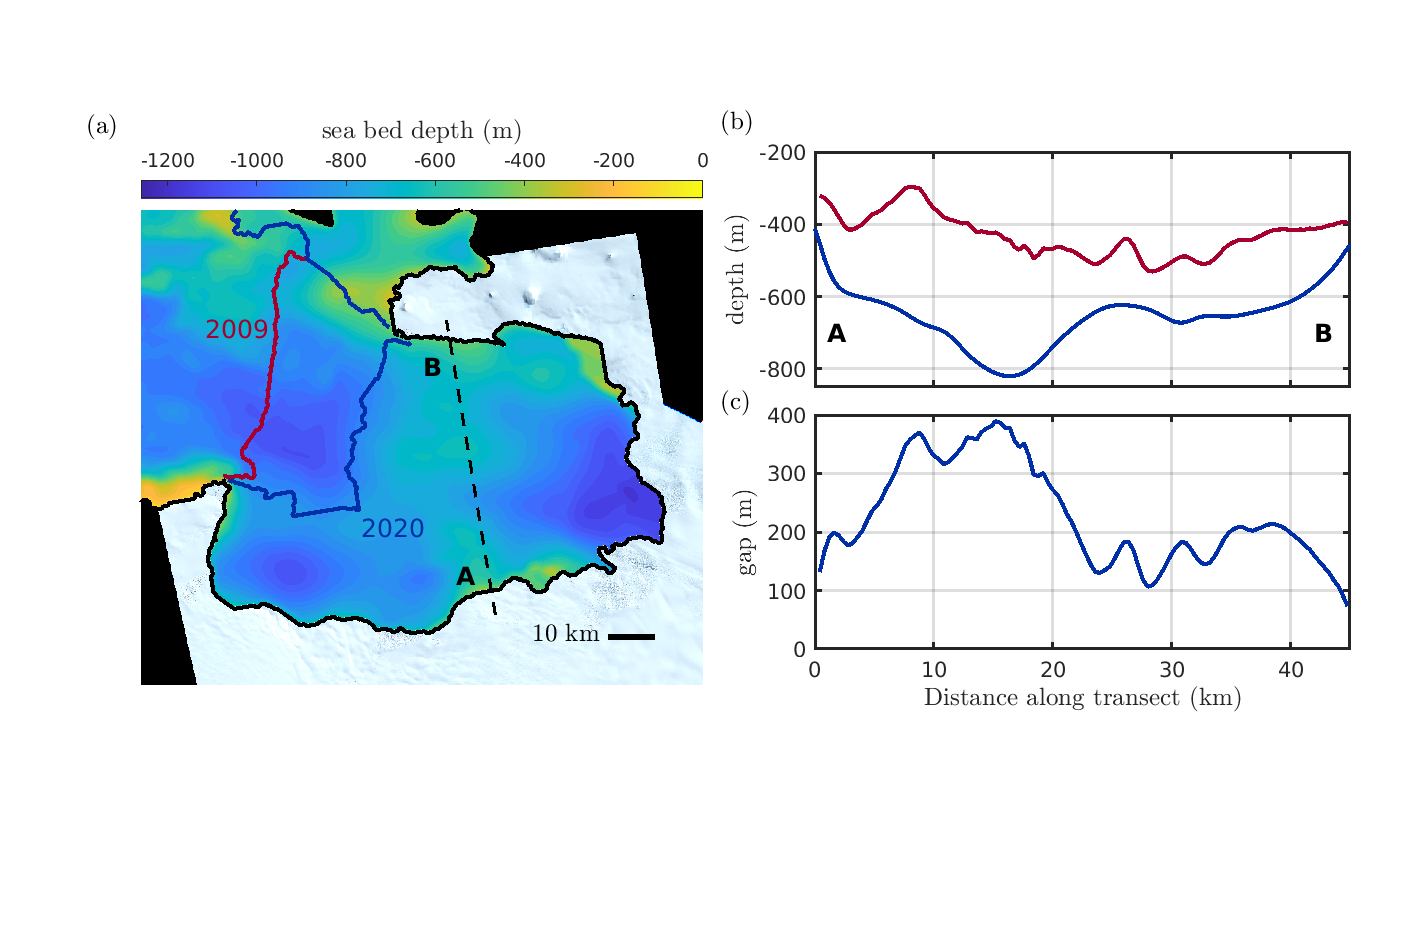
\includegraphics[width = \textwidth]{../make_figures/plots/figure1_cropped.pdf}
    \caption{(a) Contour plot of seabed depth under Pine Island ice shelf and in Pine Island Bay (colours) alongside the location of the ice front in 2009 (red line) and 2020 (blue line), as indicated. The solid black line indicates the grounding line from \citeA{Joughin2010GRL}, and the background image is a Sentinel 2 mosaic from November 2020. The black dashed line indicates the approximate location of the crest of the seabed ridge. (b) Seabed bathymetry (blue) and ice draft (red) taken along the dashed line in (a). (c) Plot of the ridge-seabed gap measured along the dashed black line in (a) (i.e. the difference between the red and blue lines in (b)). }
    \label{fig:figure1}
\end{figure}


%ridge in PIG makes pycnocline picture more complicated
For Pine Island specifically, this simple `pycnocline depth' picture is complicated by the presence of a seabed ridge in the ice shelf cavity. This ridge is located several tens of kilometers downstream of the grounding line, and protrudes up to three hundred meters above the neighboring seabed (figure~\ref{fig:figure1}). In combination with the ice shelf directly above it, the ridge acts as a topographic barrier that restricts the access of CDW to an inner cavity that has formed between the ridge and the grounding line, since the ice shelf grounding line likely retreated from this ridge in a process initiated in the late 1940s~\cite{Jenkins2010NatureGeo, DeRydt2014JGeophysResOceans, DeRydt2016JGeophysResEarthSurf, Smith2017Nature}. This cavity geometry means that the strength of the topographic barrier (i.e. how much its presence affects sub-shelf melting) is strongly dependent on the pycnocline depth: at its shallowest, the pycnocline sits above the depth of the ridge crest, and a large amount of modified CDW is able to spill into the inner cavity~\cite{Dutrieux2014Science}; in contrast, at its lowest, the pycnocline sits some way below the ridge crest and CDW access is severely restricted.  As a result, melting of Pine Island Glacier has a particularly strong sensitivity to hydrographic conditions in Pine Island Bay: \citeA{Dutrieux2014Science} reported that the total freshwater flux from the fast flowing part of Pine Island Glacier in 2009 (80~km\textsuperscript{3} year\textsuperscript{-1}), when the pycnocline was at its second-highest level on record, was more than double its value in 2012 (37~km\textsuperscript{3}~year\textsuperscript{-1}), when the pycnocline was at the second-lowest recorded depth~\cite{Webber2017NatureComms}.

%another thing we have seen is significant calving events
In addition to its unique topographic control on melt rates, the recent calving of PIIS also stands out amongst Amundsen Sea terminating ice shelves. Mass losses from ice sheets in Antarctica are dominated by calving and melting~\cite{Rignot2013Science}; in equilibrium, these losses must balance the upstream accumulation of ice. The recent retreat of ice front of PIIS, however, suggests that the calving rate is far higher than would be required to maintain an equilibrium: the ice front retreated approximately 26 km between 2009 and 2020 (figure~\ref{fig:figure1}), with the majority of this retreat happening over the period 2015--2020~\cite{Lhermitte2020PNAS, Joughin2021ScienceAdv}. This corresponds to a more-than-doubling of the calving rate, from approximately 4~km~year\textsuperscript{-1} prior to 2015 to approximately 9~km~year\textsuperscript{-1} in the period 2015--2020 (the flow speed at the ice front, for context, is approximately 5~km~~year\textsuperscript{-1} \cite{Joughin2021ScienceAdv}).

%at present, the ridge is located approx x km downstream of the ridge crest. The changes some far have been implicated in a speed up because of a loss of buttressing, but might the changes have also led to a relaxation of the topographic barrier and thus and increase in melt rates (that would only be evidenced on longer timescales(?)) [key question one]
As of 2020, the ice front is located approximately 20~km downstream of the ridge (figure~\ref{fig:figure1}); the ice front is now closer to the ridge crest than the location of the ice front in 2009. The loss of buttressing associated with this retreat has been shown to be responsible for the acceleration of PIG since 2015~\cite{Joughin2021ScienceAdv}. However, given that the topographic barrier to CDW relies on the combination of ice draft \textit{and} seabed ridge, the recent calving events beg the following question: have recent calving events relaxed the topographic barrier, leading to significant changes in melting in PIIS? Increased melting of ice shelves will lead to further reductions in ice shelf volume and thus buttressing, ultimately leading to ice shelf acceleration, thinning and grounding line retreat.

%but also, in future, we might have further calving events because or preconditioning and or MICI that might bring to ridge to the crest. How might these potential future calving events lead to changes in melt rates? [key question two]
In addition to considering the effect on melt rates of calving events that have already happened, we also consider how melt rates might respond to possible future calving events. It has been suggested that further significant calving of PIIS is inevitable: damage to the ice shelf that has already occurred is thought to have preconditioned PIIS to collapse~\cite{Lhermitte2020PNAS}. Additionally, there is a theoretical feedback loop in which damage leads to calving, reducing buttressing, leading to acceleration of the ice and thus further damage; we expect further calving as part of this feedback process that also interacts with unbalanced melting. The second question we aim to answer in this paper regards the melt response to calving in the future: how will melt rates on PIIS response to possible future calving events?

In this paper, we use numerical simulations in both an idealized domain whose geometry captures the essential features of PIG, and a realistic geometry that closely matches real world conditions for PIG to assess how, and why, melt rates in PIIS will respond to past and potential future calving events. We begin in \S\ref{S:Experiment} with a description of the experiments using the idealized geometry, setting out details of the ocean model used and the experimental setup. We perform a total of nine idealized experiments; results of one such experiment (the `baseline') are presented in \S\ref{S:Baseline}: we describe how and why the melt rate responds to calving in this experiment. In the following two sections, we discuss how the picture presented in \S\ref{S:Baseline} changes for different cavity geometries (\S\ref{S:Results:H}) and hydrographic forcings (\S\ref{S:Results:P}). In \S\ref{S:Realistic}, we describe and present results from the realistic experiments. Guided by the results of the idealized experiments, we assess the expected response of melt rates under PIIS to calving events. In \S\ref{S:Discussion}, we discuss the implications of our results and summarize the key results of the paper in \S\ref{S:Summary}.


\section{Idealized Experiment Details}\label{S:Experiment}
%broad overview of the experiemnts
In this section, we describe the setup of the experiments performed in an idealized domain whose geometry captures the essential features of the cavity under PIIS -- most notably, the presence of a seabed ridge. We refer to the experiments henceforth as `idealized experiments'. In this idealized geometry, the gap between the ice draft and the seabed ridge (the `ridge-draft' gap) is uniform in the zonal direction. In practice, however, the ridge-draft gap is non-uniform (figure~\ref{fig:figure1}); to capture the effect of this variation, we consider the melt response to calving for several different ridge-draft gaps. We also consider several different far-field ocean conditions (`hydrographic forcings'): as discussed in \S\ref{S:Introduction}, melt rates on PIIS have a sensitive dependence on the hydrographic forcing via the depth of the pycnocline; we therefore expect that the melt response to calving might similarly have a sensitive dependence on the hydrographic forcing, and investigate this effect.

The benefit of considering first idealized experiments is that, by simplifying the cavity geometry, we are able to isolate the important roles that the ridge-draft gap and the hydrographic forcing play in the melt response to calving in a cavity with a topographic barrier that prevents warm water from reaching an inner cavity, as well as elucidating the physical mechanisms responsible for these changes. 

We perform a total of nine idealized experiments, each corresponding to a unique pair of parameters that describe the ridge-draft gap and the hydrographic forcing; these parameters are described in sections \S\ref{S:Experiment:Geometry} and \S\ref{S:Experiment:Hydrography}, respectively. Each experiment consists of a series of ten simulations in which the ice front position is systematically reduced; we use the term calving as a proxy for this process, but stress that our simulations include neither calving dynamics nor associated processes such as mélange formation. In each simulation, we explicitly resolve the ocean circulation using the MIT general circulation model (MITgcm)~\cite{Marshall1997JGROceans}. Other than removing sections of the ice shelf, the ice shelf geometry does not change within each experiment. Ice shelves themselves enter the ocean model passively, via the exchange of heat and salt at the ice-ocean interface and a steady pressure loading on the ocean surface (i.e. there are no ice-dynamics considerations in the cavity geometry); a passive description of ice shelves is sufficient to assess the response of melt rates to ice shelf calving, which occurs on a timescale much shorter than that on which the ice responds dynamically to perturbations in melting. In the following sections, we provide further details of the ocean model and experimental setup, including the motivation for our choices of parameters.


\subsection{Details of Ocean Model}\label{S:Experiment:Model}
The MITgcm is a z-level general circulation model that includes a partial-cell treatment of topography, allowing an accurate description of both the seabed and ice draft. Our model grid consists of 110 layers with a vertical spacing of 10~m, and a horizontal resolution of 400~m. We use the MITgcm in hydrostatic mode with an implicit nonlinear free surface scheme, a third-order direct space-time flux limited advection scheme, and a non-linear equation of state~\cite{Mcdougall2003JAtmosOceanTech}. The Pacanowski-Philander \cite{Pacanowski1981JPhysOcean} scheme parametrizes vertical mixing. Constant values of 15 and 2.5 
m\textsuperscript{2} s\textsuperscript{-1} are used for the horizontal Laplacian viscosity and horizontal diffusivity, respectively. The equations are solved on an $f$-plane with $f = -1.4\times10^{-4}~\text{s}^{-1}$.

Each simulation is run for twelve months using a timestep of 30~\si{seconds}, after which time the configuration is approximately in steady state. The melt rates are within 95\% of their final values after three months. All results presented here are averaged over the final two months of the simulations.

As mentioned, ice shelves enter the simulations via the exchange of heat and salt at the ice-ocean interface. This exchange is implemented using the so-called "three-equation formulation"~\cite{Holland1999JPhysOcean}, whose implementation in MITgcm has been described in detail elsewhere \cite[for example]{Losch2008JGeophysResOceans, DeRydt2014JGeophysResOceans,Dansereau2014JGROceans}. Note that the temperature difference between ice shelves and the adjacent ocean boundary layer is one to two orders of magnitude smaller than the temperature associated with phase changes -- $L/c \approx -84\si{\Celsius}$, where $L=3.35\times10^5$ is the latent heat of fusion, and $c_p=3947~\si{\joule \kilogram}^{-1}$ is the specific heat capacity of water. Thus, thermal exchange across the ice-ocean interface is typically dominated by latent heat (over heat conduction into the ice). With latent heat dominated thermal exchange, the three equation formulation simplifies to give the melt rate $\dot{m}$ as
\begin{equation}\label{E:MeltRate}
    \dot{m} = \frac{c_p \gamma_T (T - T_b)}{L}.
\end{equation}
Here $T$ is the temperature far outside the viscous boundary layer that forms at the ice-ocean interface, $T_b$ is the temperature at the ice shelf base, which must be at the local (depth and salinity dependent) freezing point, and $\gamma_T$ is a heat exchange co-efficient that parametrizes exchange across this boundary layer. The heat exchange-coefficient $\gamma_T$ has a weakly non-linear relationship on $u^*$, the ocean speed adjacent to the ice shelf base~\cite{Holland1999JPhysOcean}; if this relationship were perfectly linear, $\gamma_T \propto u^*$, equation~\eqref{E:MeltRateUdT} would read
\begin{equation}\label{E:MeltRateUdT}
    \dot{m} \propto u^* (T - T_b).
\end{equation}
We shall return to equation~\eqref{E:MeltRateUdT} when describing the mechanisms responsible for melt rate variation with ice shelf calving.

We use parameter values from \citeA{Holland1999JPhysOcean} in the three equation formulation, with the exception of the drag co-efficient, which is set to $4.5\times10^{-3}$, a value that is more appropriate for Pine Island Glacier (see \S\ref{S:Realistic}). (Note that the drag coefficient that enters the momentum balance, which can be set independently, remains at the standard value of $2.5\times 10^{-3}$.)

\begin{figure}
    \centering
    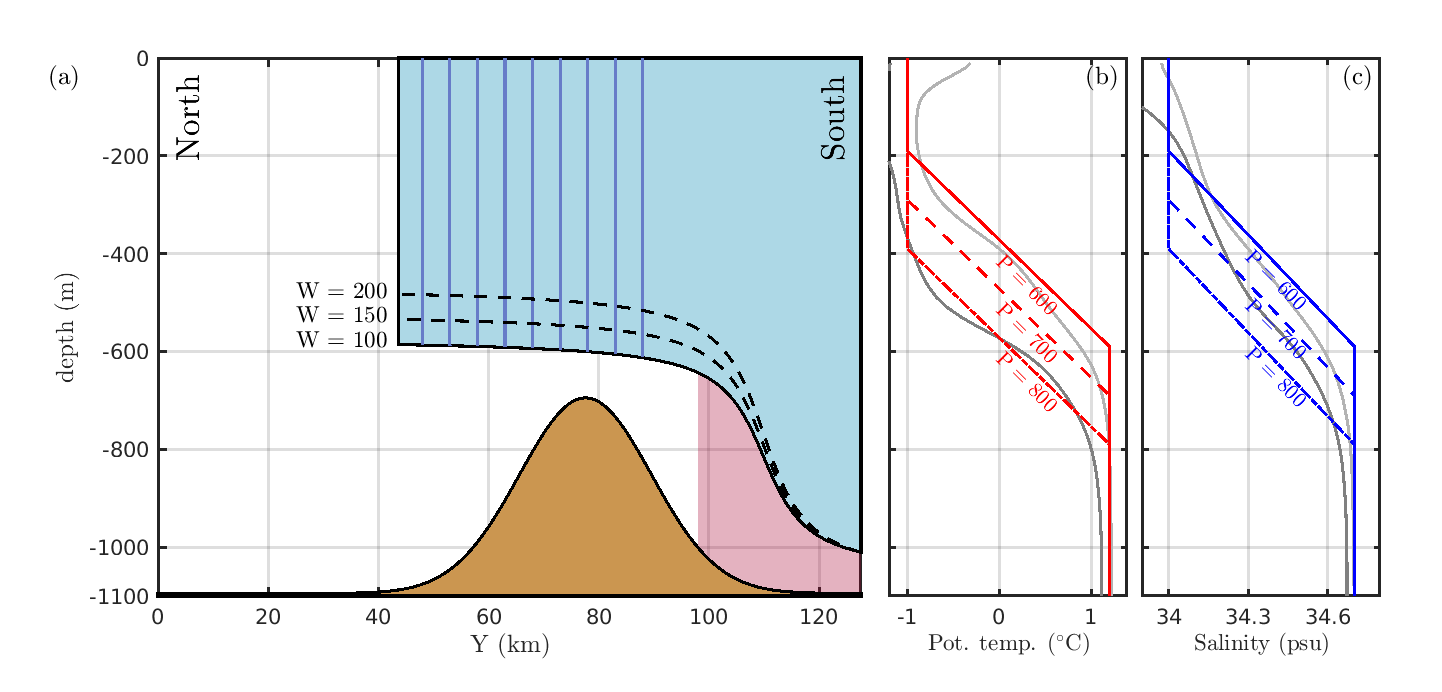
\includegraphics[width = \textwidth]{../make_figures/plots/figure2.eps}
    \caption{(a) Schematic diagram of the experimental setup. The domain is uniform in the zonal direction (into the page), with extent 48~km. The ocean domain consists of the gridded area, which is bordered by a passive ice shelf (shaded blue) and a seabed ridge (shaded brown). Solid, dashed and dot-dashed black curves indicate the location of the ice shelf base for $W$=100~m, $W$=150~m, and $W$=200~m, respectively (as labelled). Solid blue lines indicate the series of ice front positions considered within each `calving' experiment, located at 80, 75, 70, 65, 60, 55, 50, 45, and 40~km offshore of the southern end of the domain. The shaded red region indicates the inner cavity, defined as areas within 30~km of the southern end of the domain. (b) Temperature and (c) salinity profiles used in the experiments. Different line styles correspond to different values of the pycnocline depth $P$ as follows: $P$=600~m (solid), $P$=700~m (dashed), $P$=800~m (dot-dashed). Light and dark gray lines correspond to temperature and salinity profiles taken from conductivity, temperature, and depth measurements in Pine Island Bay during the austral summers of 2009~\cite{Jacobs2011NatureGeosci} and 2012~\cite{Dutrieux2014Science}, respectively.}
    \label{fig:figure2}
\end{figure}

\subsection{Ice Shelf Geometry and Seabed Bathymetry}\label{S:Experiment:Geometry}
Our idealized setup is shown schematically in figure~\ref{fig:figure2}a: it is uniform in the zonal direction, along which the $x$-axis is aligned, and the $y$-axis is aligned along the meridional direction. Note that although PIG is aligned approximately east-west, we assume here that it is aligned north-south, as is standard~\cite{Grosfeld1997JGROceans, DeRydt2014JGeophysResOceans}.

The sea bed has a Gaussian profile,
\begin{equation}\label{E:Experiment:Bed}
    b(x,y) = -1100 + 400 \exp\left[-\frac{\left(y - 50\times 10^3\right)^2}{2\sigma^2}\right],
\end{equation}
where $\sigma = 12$~km is the length scale over which this profile decays towards zero. The profile~\eqref{E:Experiment:Bed} corresponds to a ridge that peaks at a height of 400~m above the surrounding bathymetry. This peak occurs 50 km from the southern end of the domain, which we consider as the grounding line (note that we prevent the cavity thickness from reaching zero at this `grounding line' as the MITgcm requires at least two grid cells in the vertical to permit horizontal transfer). 

The variability in both PIIS draft and the height of the seabed ridge result in a ridge-draft gap that varies between approximately 100 m at its narrowest to greater than 300 m at its widest (figure~\ref{fig:figure1}b,c). Since we use the same seabed geometry (and, in particular, the same ridge height) in each simulation, we aim to gain insight into the effect of variation in the ridge-draft gap by considering several different values of $W$ -- the vertical distance between the crest of the seabed ridge and the ice shelf base (figure~\ref{fig:figure2}a). $W$ enters only the model only via the ice profile; following~\citeA{DeRydt2014JGeophysResOceans}, we use an ice shelf draft that is given by
\begin{equation}
    h(y) = \begin{cases}
    \left(\frac{310 + W}{2.64}\right)\tan^{-1}\left(\frac{y}{5882} -3\right) & \text{for}~y < y_f,\\
    0  & \text{for}~y \geq y_f.
    \end{cases}
\end{equation}
Here $y_f$ is the variable location of the ice front (see below). We stress that these ice profiles are not obtained from ice dynamics considerations, but selected for their qualitative similarity to PIIS: they include a flatter section offshore of the ridge and a steeper section inshore of the ridge that is observed in practice (figure~\ref{fig:figure2}a).

We consider three different values of $W$ here: $W$=100~m, $W$=150~m, and $W$=200m. The smallest value, $W = 100$m, corresponds to the minimum observed ridge-draft gap in Pine Island (figure~\ref{fig:figure1}b,c), while the largest value, $W$=200m, corresponds to an upper bound, beyond which there is little melt response to calving, as we shall see. 

Within each experiment, the front position $y_f$ is systematically reduced, as a proxy for calving. The ten simulations within each experiment use values $y_f$=84, 80, 75, 70, 65, 60, 55, 50, 45, and 40~km, which correspond to calved lengths of $l_c$=0, 4, 9, 14, 19, 24, 29, 34, 39, and 44~km, respectively. Within each experiment, the simulation with $y_f$ = 84~km is referred to as the `uncalved' simulation, serving as a benchmark against which results are compared. There are both pragmatic and physical reasons for choosing this particular range of values for $y_f$: the uncalved simulation corresponds roughly to the observed distance of the ice front from the PIG grounding line in 2009, before significant calving took place in the late 2010s; the lowest value, $y_f$ = 40~km, is chosen as a compromise between allowing us to consider scenarios in which the ice front has been retreated significantly beyond the ridge, whilst retaining a large area that is shared by each experiment (as we discuss further in \S\ref{S:Baseline}, the area over which melt rates are averaged must be invariant to calving for a robust assessment of the melt response to calving). The computational expense of high resolution ocean simulations forces us to restrict the number of simulations within each experiment to ten.


\subsection{Hydrographic Forcing}\label{S:Experiment:Hydrography}
For each unique value of $W$, we perform each of the three, each with a different hydrographic forcing. Comparing the results of these experiments gives us an indication of the sensitivity of our results to hydrographic forcing. The range of these hydrographic forcings covers that which is observed in practice (see below).

The hydrographic forcing is imposed on the model by means of a restoring boundary condition at the northern end of the domain: at this boundary, the temperature and salinity are restored to specified vertical profiles, shown in figure~\ref{fig:figure2}b,c, over a distance of five horizontal grid cells (total length 2 km) with a restoring timescale that varies from 12~hours at the boundary to 60~hours at the interior of this restoring regions. (The model includes solid walls with a free slip condition at the southern, western, and eastern sides of the domain.) These temperature and salinity profiles are piecewise linear functions of depth: they are constant in both an upper (temperature $-1^\circ$C, salinity $34$~psu) and lower layer (temperature $1.2^\circ$C, salinity $34.7$~psu), which are separated by a pycnocline of thickness 400~m across which the temperature and salinity vary linearly. The pycnocline begins at a variable depth $P$ (a higher $P$ corresponds to a deeper pycnocline), which parametrizes the whole profile (figure~\ref{fig:figure2}b,c); the three hydrographic forcings we consider have $P$=600 m, 700 m, and 800 m. 

%why do we choose these conditions
These piecewise linear profiles are approximations to typical conditions for Pine Island Bay~\cite{Jacobs1996GRL, Dutrieux2014Science, Jenkins2018NatureGeo} (see figure~\ref{fig:figure2}a,b), where the upper and lower layers are primarily Winter Water and (modified) Circumpolar Deep Water, respectively. As mentioned, the record of hydrographic conditions in Pine Island Bay (PIB) has revealed significant variability in the depth of the pycnocline on interannual timescales~\cite{Dutrieux2014Science}; the profiles with $P = 600$ and $P = 800$ are approximations to profiles observed in PIB in the years 2009 and 2012, respectively. These two years approximately span the range of observed conditions: in 2009, the average depth of the pycnocline was at its shallowest level on record, while in 2012, the average depth of the pycnocline was at its second-deepest level on record (the lowest pycnocline depth, recorded in 2013, was only marginally lower than in 2012~\cite{Webber2017NatureComms}).

%wrap up the experiments:\ 
The nine experiments are uniquely identified by a $(W,P)$ pair, where $W$ $\in \{100, 150, 200\}$~m and $P$ $\in \{600, 700, 800\}$~m. We consider the extreme scenario with the strongest topographic barrier and the hydrographic forcing with the thickest CDW layer, $(W,P) = (100,600)$~m to be the baseline experiment, against which the other experiments are compared; in the following section, we describe the results of the baseline experiment, before describing in sections~\ref{S:Results:H} and~\ref{S:Results:P} how this picture changes for different values of $W$ and $P$, respectively.


\section{Results for the Baseline Experiment ($H$=100~m, $P$=600~m)}\label{S:Baseline}
In this section, we describe the results for the baseline experiment with $W$ = 100~m and $P$ = 600~m (solid lines in figures~\ref{fig:figure2}a--c). We begin by describing the steady state ocean configuration in the uncalved simulation, and then describe how, and why, the melt rate responds to calving.

\subsection{Uncalved Simulation}\label{S:Baseline:Default}
\begin{figure}
    \centering
    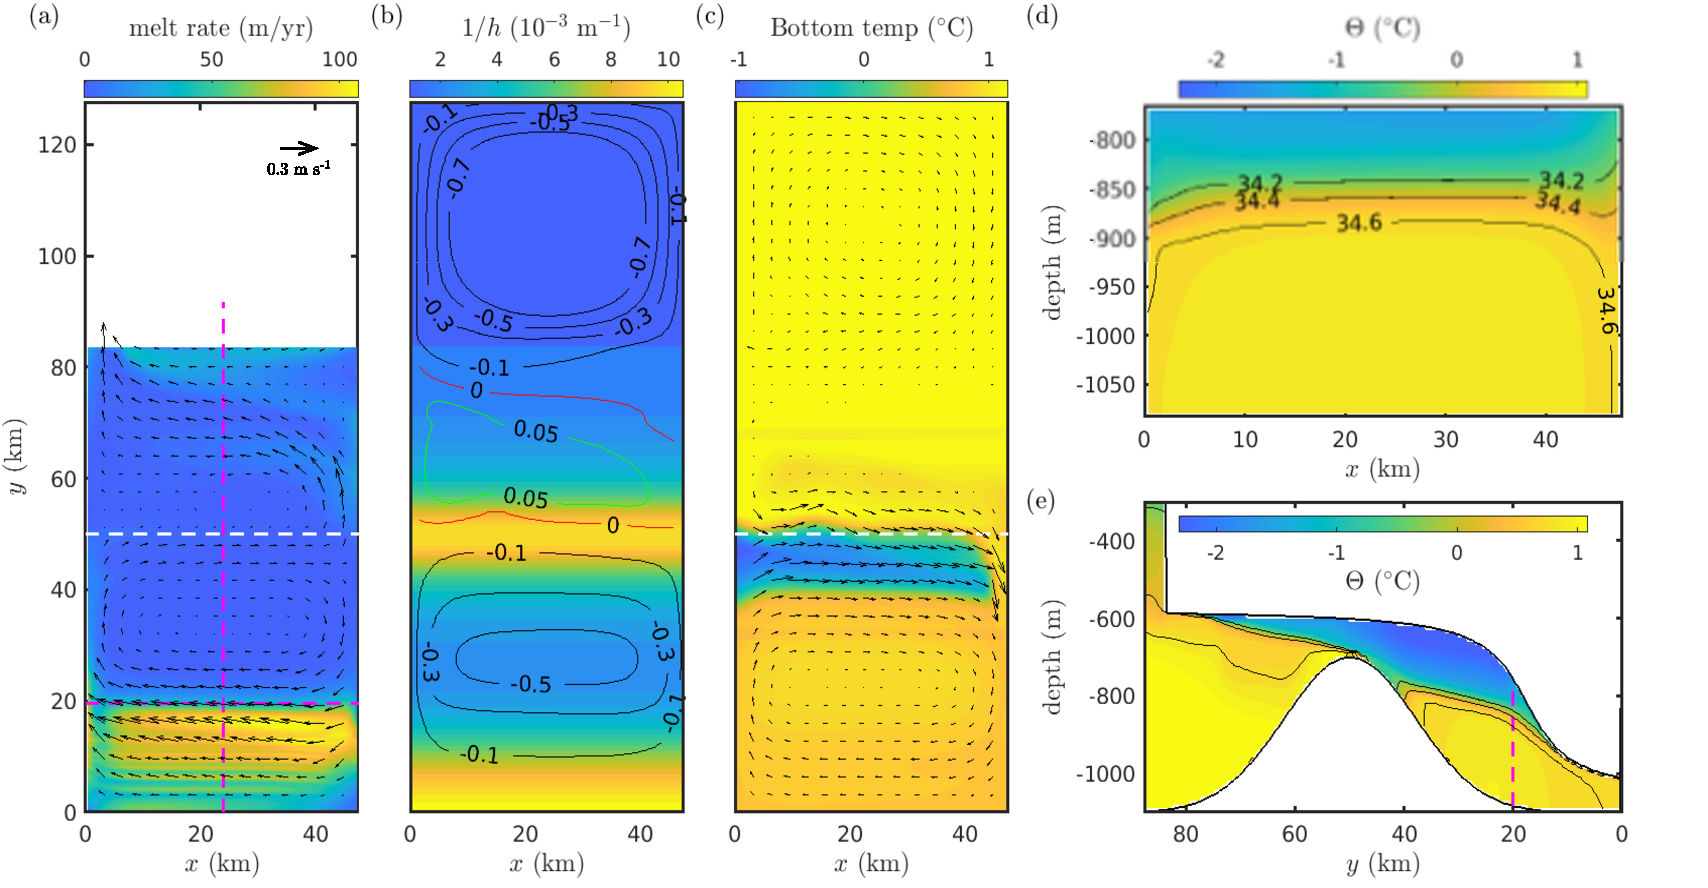
\includegraphics[width = \textwidth]{../make_figures/plots/figure3-with-arrow.pdf}
    \caption{Ice-ocean properties that characterize the default (uncalved) simulation in the baseline experiment ($W$ = 100~m, $P$ = 600~m). (a) Melt rate (colours) and boundary layer velocities (arrows, every fifth velocity vector is plotted), averaged over the three grid cells adjacent to the ice-ocean interface. White areas correspond to open ocean. The black line indicates an arrow length that would correspond to 0.6~m~s\textsuperscript{-1}. The white dashed line indicates the location of the top of the ridge (along which the section in (d) is taken) and the magenta dashed line indicates the meridional centre line (along which the section in (e) is taken). (b) Inverse water column thickness $1/h$ (colours) and barotropic stream function (black contours, in units of Sv). Note that only contour levels 0, -0.1, -0.3, -0.5, and -0.7~Sv are shown. (c) Bottom temperature (colours) and bottom current (arrows) averaged over the three grid cells closest to the seabed. The scale bar for velocity vectors in (a) is also appropriate for (c). (d) Zonal cross-section taken along the ridge crest (white dashed line in (a)) up to the ice shelf base, showing potential temperature (colours) and salinity contours at the 34.2, 34.4, and 34.6~psu levels. (e) Meridional cross-section, taken along the magnenta dashed line in (a), with colours and contours as in (d).}
    \label{fig:figure3}
\end{figure}

%describe each of what we see: melt rate, general observations
Ice-ocean properties that characterize the default simulation are shown in figure~\ref{fig:figure3}. Melt rates (figure~\ref{fig:figure3}a) are below  20~m~year\textsuperscript{-1} everywhere, except for a region located within 20~km of the grounding line, where melt rates reach a maximum of approximately 120~m~year\textsuperscript{-1}. The average melt rate over the whole shelf is approximately 20~m~year\textsuperscript{-1}; this is lower than the value of 33$\pm$2~m~year\textsuperscript{-1} that was estimated by~\citeA{Jenkins2010NatureGeo} based on observations in Pine Island Bay in 2009 (to which the $P=600$ case corresponds). This discrepancy is expected, given that this simulation corresponds to the extreme scenario in which the ridge-draft gap is set to the minimum gap that is observed in practice.

%introduce the idea of the inner cavity, why do we use this metric
At this point, we introduce the definition on the `inner cavity' as the area of the ocean that is located within 30~km of the Southern end of the domain (red shaded region in figure~\ref{fig:figure2}a). We use the mean melt rate in the inner cavity, referred to as the `inner cavity melt rate', as a single metric to quantify changes in melt rate with calving. Since the melt rate is highly spatially variable (figure~\ref{fig:figure3}a) it is necessary to consider a fixed area, which is common to each simulation, when assessing changes in melt rate with calving. This best demonstrated by example: integrating over the whole shelf, for example, would make smaller shelves appear to have anomalously large melt rates, since the region of high melt close to the grounding line would occupy a greater proportion of the total shelf. %A spatially invariant area over which the melt rate is integrated is necessary because the melt rate under the ice shelf is highly spatially variable (figure~\ref{fig:figure3}a); for example, if we removed sections of ice in the default run \textit{without} changing the melt rate pattern, those runs with less ice (i.e. significant calving) would display larger mean melt rates over the whole shelf because the highest melt rates are concentrated near the grounding line.
The choice of 30~km in defining the inner cavity region reflects a compromise between including simulations in which the ice front is receded a significant distance beyond the ridge (the smallest shelf we consider must be larger than the inner cavity region), while including a reasonably large section of the uncalved ice shelf over which the melt rate is averaged. Crucially, this choice of inner cavity includes the grounding line, a region in which changes in melt rate are acutely important for the dynamics of the ice sheet \cite{Seroussi2014Cryo, Athern2017GRL}. Although the values of inner cavity melt rate \textit{are} dependent on the particular definition, we verified that the trends and key results are independent of the choice of inner cavity. The inner cavity melt rate in the uncalved run ($l_c$=0~km) is 46\mpryr (figure~\ref{fig:figure3}a).

%why does the melt rate look like it does
Melt rates depend on both the cavity circulation and thermal driving (see equation~\eqref{E:MeltRate}). Cavity circulation (figure~\ref{fig:figure3}a,c) is characterized by a Coriolis-drive cyclonic circulation. This circulation is directed northward at the eastern boundary ($x$=0~km) and southward at the western boundary ($x$=48~km). In the inner cavity, the circulation is vigorous South of $y$=30~km, but high melt rates are restricted to $y<$ 20~km: north of $y$=20~km, a cold and fresh meltwater plume sits adjacent to the ice-ocean interface (figure~\ref{fig:figure3}e) and the thermal driving is therefore much smaller than in $y<$20~km, where the ice is adjacent to warm water.


%we can use the bsf 
\rout{To understand this pattern of melt rates, it is instructive to consider the barotropic stream function (figure~\ref{fig:figure3}b). In general, if the circulation is geostrophic, with buoyancy driving force balancing Coriolis forces, the flow will be barotropic and the velocity will align with contours of constant $f/h$, where $h$ is the water column thickness; in this idealized domain, contours of constant water column thickness correspond to lines of constant $y$, aligned East-West. There are two main potential vorticity (PV) barriers, where the water column thickness changes rapidly, forcing the flow to be diverted: the first is at the ice front, where high fluid velocities associated with the resulting divergent current lead to locally enhanced melt rates of up to 50\mpryr (figure~\ref{fig:figure3}a). The second is at the seabed ridge. As flow approaches the ridge, it is diverted Eastward (figure~\ref{fig:figure2}a) to retain a constant PV. Ultimately, the PV barrier in this `narrow gap' case is sufficiently strong that little flow is able to penetrate across the ridge (note the zero barotropic contour at the top of the ridge in figure~\ref{fig:figure3}b). The exception to this is a strong boundary current at the East, where flow divergence and relative vorticity permit flow perpendicular to contours of constant column this thickness, which is Southward (Northward) in the East (West). As a result of this PV barrier, a strongly topographically constrained circulation spins up inshore of the ridge.} %, a feature that is common to more realistic simulations of Pine Island~\cite{Heimbach2012AnnGlac, Dutrieux2014Science}.

\textcolor{blue}{To understand this pattern of melt rates, it is instructive to consider the barotropic stream function (figure~\ref{fig:figure3}b). Although the buoyancy driving means that the flow is not purely barotropic, the barotropic component makes up a significant component of the flow [show this]. In the case that the flow is entirely barotropic, it will conserve its potential vorticity: assuming that turbulent stresses and viscous stresses are negligible, the barotropic component of flow must conserve the shallow-water potential vorticity (PV) $(f + \zeta)/h$, where $h$ is the water column thickness and $\zeta$ is relative vorticity. Flow must align with $f/h$ contours, or gain a relative vorticity; in this idealized domain, contours of constant water column thickness correspond to lines of constant $y$, aligned east-west. The seabed ridge provides the main PV barrier. As flow approaches the ridge, it gains relative vorticity and is diverted eastward  (figure~\ref{fig:figure2}a). Ultimately, however, the PV barrier in this `narrow gap' case is sufficiently strong that little flow is able to penetrate across the ridge (note the zero barotropic contour at the top of the ridge in figure~\ref{fig:figure3}b). The exception to this is a strong boundary current at the East, where flow divergence and relative vorticity permit flow perpendicular to contours of constant column this thickness, which is southward (northward) in the east (west). As a result of this PV barrier, a strongly topographically constrained circulation spins up inshore of the ridge. \textbf{Need to say something about the overturning circulation flushing the inner cavity, but not sure where that comes into this paragraph, perhaps by contrasting with above: "the baroclinic component is dominated by an overturning circulation..."}}

The connection between the inner and outer cavities comes exclusively via the boundary currents; in the central trunk, warm CDW is blocked from entering the inner cavity by \textcolor{red}{the presence of the meltwater plume, which extends from the ridge crest to the ice shelf base (figure~\ref{fig:figure3}e)} \textcolor{blue}{the potential vorticity barrier provided by seabed ridge and ice shelf draft, and the ridge hosts meltwater on the inner cavity side}. Water entering at the Eastern boundary mixes with \red{the plume} \blue{this meltwater} as it crosses the ridge; warm water that enters the inner cavity is lightly modified by this mixing, resulting in a bottom temperature that is slightly cooler (approximately 0.8${}^\circ$C) inshore of the ridge than offshore (approximately 1.3${}^\circ$C, see figure~\ref{fig:figure3}). The effect of warm water intrusion on melting is twofold: it both provides significant heat to the inner cavity, and increases the stratification and thus speed of the topographically confined (approximately geostrophic) cyclonic circulation.

In summary, in this uncalved simulation, which a strong barrier for CDW access to the inner cavity, a topographically constrained cyclonic circulation is spun up inshore of the ridge. A strong current at the Eastern boundary provides the inner cavity with lightly modified warm water. The presence of this warm waterm enhances melting by both providing more heat and resulting in a stronger circulation in the inner cavity.

%We note that despite this simulation corresponding to a topographic barrier that is expected to be stronger than reality, several features are in agreement with observations such as the presence of warm water on the inner cavity, the presence of a strong meltwater plume that is coldest inshore of the ridge, and a weak hydrographic front that forms on the Northern slope of the ridge~\cite{Jenkins2010NatureGeo}.

%figure 4: plots of (a) melt rate and velocity vectors, (b) geostrophic contours and BSF overlain and (c) bottom current and temperature (i.e. a la Jan 2014 paper)
\subsection{Calving Response}
The inner cavity melt rate as a function of the calved length $l_c$ is shown in figure~\ref{fig:figure4}. We see that, while the ice shelf front is located far offshore of the ridge ($l_c < 14$~km), removing sections of ice results in only a weak increase in the inner cavity melt rate. However, as the ice shelf front is retreated further towards the ridge, the melt rate increases dramatically, reaching a maximum of 73\mpryr (70\% larger than in the uncalved run) when the ice shelf is located approximately 5~km north of the ridge crest. Perhaps surprisingly, retreating the ice front slightly further to sit above the ridge crest results in a significant decrease in the inner cavity melt rate of approximately 15\% (from 73\mpryr to 64\mpryr). Finally, the inner cavity melt rate is approximately independent of ice front position when the ice front is located inshore of the ridge ($l_c>$34~km).

%figure 5: (a) plot of mean melt rate as a function of extent and (b) millgate decomposition 
\begin{figure}
    \centering
    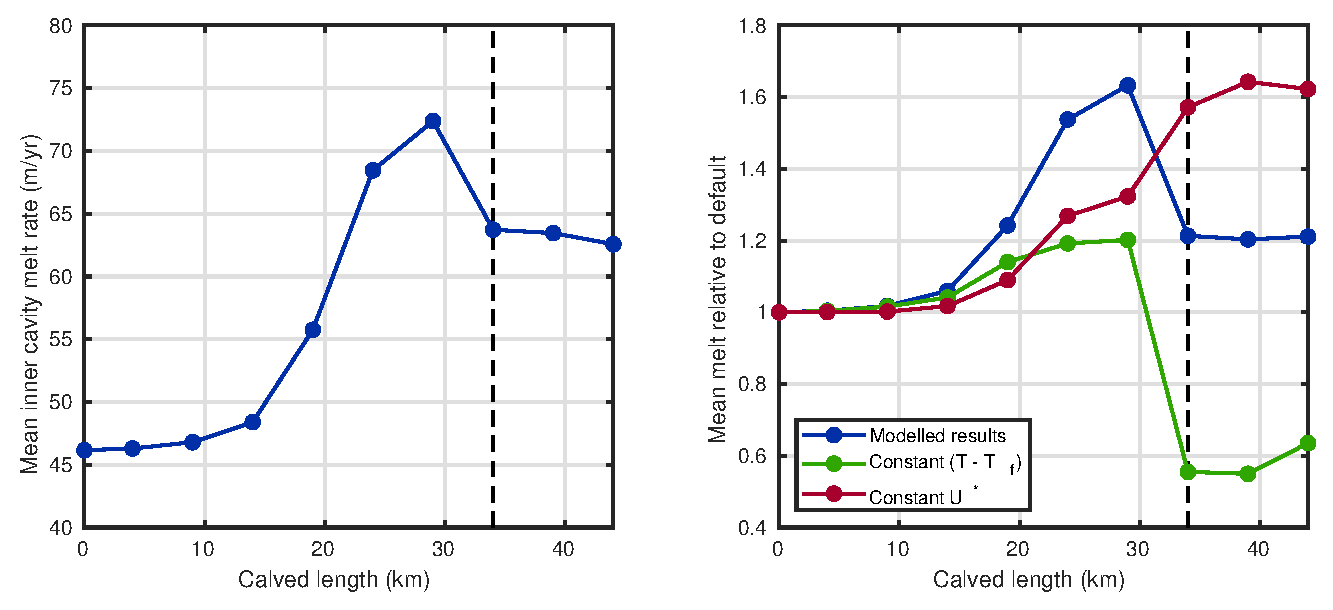
\includegraphics[width = \textwidth]{../make_figures/plots/figure4.eps}
    \caption{(a) Mean inner cavity melt rate as a function of the calved length $l_c$. The black dashed line indicates the position of the ice front when it is located directly above the seabed ridge. (b) Velocity-thermal driving decomposition: decomposition of changes in inner cavity melt rate relative to the uncalved simulation into changes in boundary layer speed $U_e$ (green curve, equation~\eqref{E:MillgateDecompU}) and thermal driving $\Delta T_e$ (red curve, equation~\eqref{E:MillgateDecompDT}). The blue curve indicates the change in melting relative to the uncalved simulation (equation~\eqref{E:MillgateDecompMelt}).}
    \label{fig:figure4}
\end{figure}

%explain what the Millgate decomposition.
To understand the reasons for this variation in melt rate with calving, it is instructive to return to equation~\eqref{E:MeltRateUdT}, which indicates that the melt rate is approximately proportional to the product of the boundary layer velocity and thermal driving. We investigate the relative roles of variations in both of these quantities in the changes to the inner cavity melt rate. To do so, we replace the boundary layer velocity and thermal driving fields in each of the simulations with the corresponding fields from the uncalved simulation, and calculate the resulting inner cavity melt rate relative to the actual inner cavity melt rate from that particular simulation~\cite{Millgate2013JGROceans}. Explicitly, the relative effect of changes in boundary layer velocity and thermal driving on the inner cavity melt rate are assessed by computing
 \begin{align}
U_{e}(l_c) &=  \int_{\text{inner cavity}}\frac{u^*(x,y; l_c)}{u^*(x,y; l_c = 0)}~\mathrm{d}x\mathrm{d}y, \label{E:MillgateDecompU}\\ \Delta T_{e}(l_c) &= \int_{\text{inner cavity}}\frac{T(x,y; l_c) - T_b(x,y; l_c)}{T(x,y; l_c = 0) - T_{b}(x,y; l_c = 0)}~\mathrm{d}x\mathrm{d}y,\label{E:MillgateDecompDT}
 \end{align}
  where $u^*(x,y;l_c = 0)$, $T(x,y,l_c = 0)$, and $T_b(x,y,l_c = 0)$ are the boundary layer velocity, ocean temperature and local freezing temperature that emerge from the uncalved simulation. The quantities in~\eqref{E:MillgateDecompU}--\eqref{E:MillgateDecompDT} are compared, for a given calved length $l_c$, to the relative change in melting over the default simulation,
 \begin{equation}\label{E:MillgateDecompMelt}
   \mathcal{M}(l_c) =  \int_{\text{inner cavity}}\frac{\dot{m}(x,y, l_c)}{\dot{m}(x,y; l_c = 0)}~\mathrm{d}x\mathrm{d}y.
 \end{equation}
The quantities~\eqref{E:MillgateDecompU}--\eqref{E:MillgateDecompMelt} are plotted in figure~\ref{fig:figure4}b as a function of $l_c$.  Here, a melt response to calving that results exclusively from changes in the thermal driving would be indicated by indistinguishable blue and red curves, and a green curve that always takes the value one, while a melt response that results exclusively from changes in boundary layer velocity would be indicated by indistinguishable blue and green curves, and a red curve that always takes the value one. We refer to this comparison as a `velocity-thermal driving decomposition' henceforth. %(Note, however, that while the relative change in melt rate depends on the changes in velocity and thermal driving, this relationship is not linear.) 



%what do these plots tell us about what is responsible for the changes?
The velocity-thermal driving decomposition (figure~\ref{fig:figure4}b) indicates that both changes in the boundary layer velocity and thermal driving play an important role in the melt response to calving in this experiment (i.e. neither plays a dominant role).  When the ice front is located offshore of the ridge ($l_c < 25$~km), ice front retreat results in increases in both the boundary layer velocity and thermal driving; these increases are complimentary: they act in unison to increase the inner cavity melt rate with calving. When the calving front is retreated to sit above the ridge, the thermal driving effect increases further, while the velocity effect decreases sharply, indicating that a significant slowing down of the inner cavity circulation takes place at this point; further, this slowing of the cavity circulation outweighs the increase in thermal driving, leading to an overall reduction in the inner cavity melt rate when front is retreated to sit directly above the ridge. 

%figure 6:  (a) row of melt rate (colours) and BSF contours, (b) zonal sections, (c,d) meridional sections
\begin{figure}
    \centering
    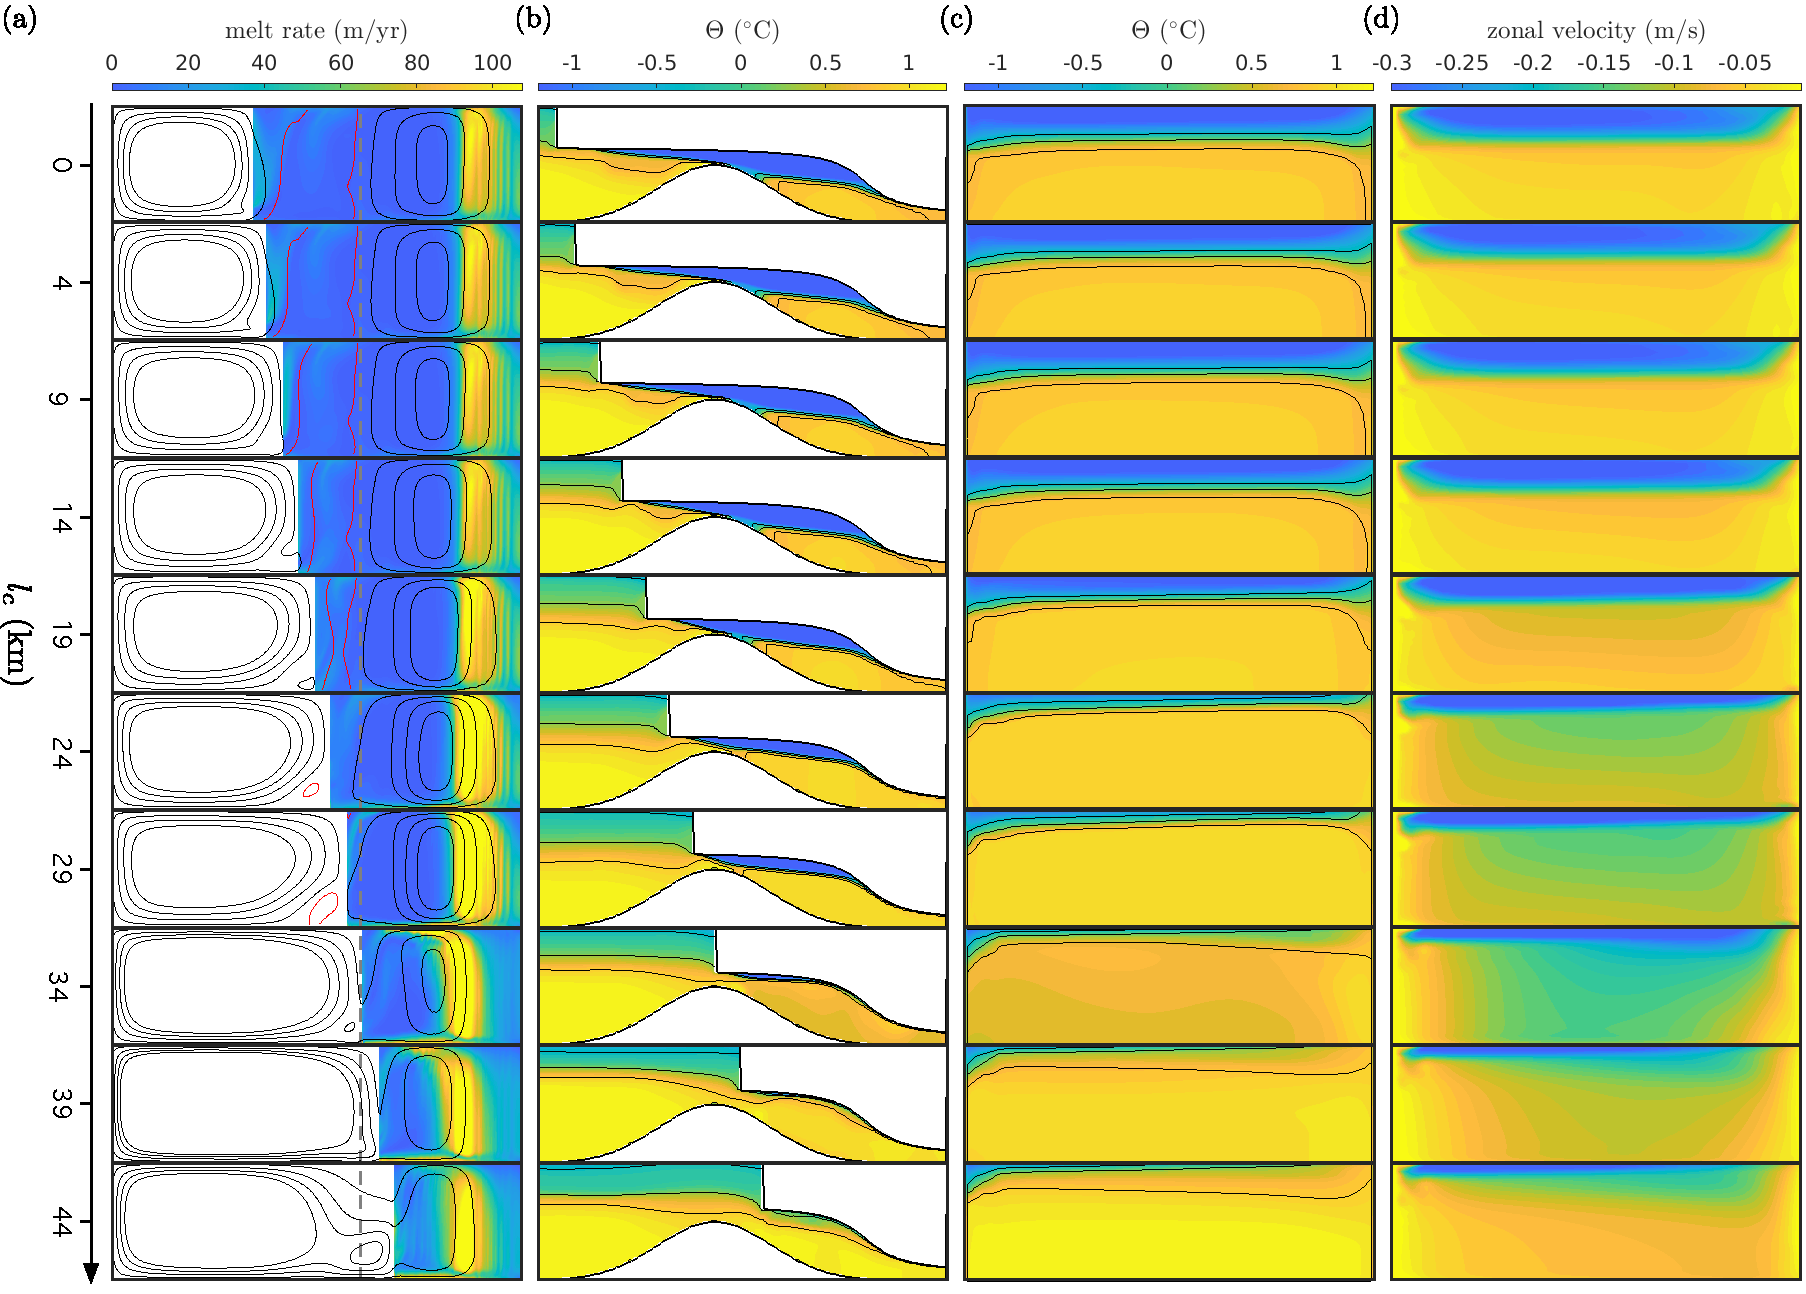
\includegraphics[width = 0.99\textwidth]{../make_figures/plots/figure5_axislabel.pdf}
    \caption{(a) Contour plots of melt rate (colours) and barotropic stream function (contours, black at 0.1, 0.3, 0.5, and 0.7 Sv levels and magenta at the 0~Sv level) in the idealized simulation with $P$ = 600~m and $W$ = 100~m. The calved length $l_c$ increases from 0~km in the first row to 44~km in the final row. The white sections indicate open ocean. (b) Contour plots of potential temperature $\Theta$ (colours) and salinity (contours, at levels 34.2, 34.4, and 34.6~psu, as in figure~\ref{fig:figure3}, black arrows indicate the direction of increasing salinity) taken along the centreline of the domain (magenta dashed line in figure~\ref{fig:figure3}a). The white section at the top and bottom of each subplot indicate the ice shelf and seabed ridge, respectively. (c) Contour plots of potential temperature (colours) and salinity (contours, at levels 34.2, 34.4, and 34.6~psu) along a zonal section located 20~km downstream of the grounding line. (d) As in (c) with colours indicating the zonal velocity.  In each case, the colour bar at the top of the column is appropriate for each row in the column. (Note that the first row in columns (a), (b), and (c) in the first row show the same data as in figure~\ref{fig:figure3}(a), (d), and (e), respectively.) }
    \label{fig:figure5}
\end{figure}

%how can we understand what happens.
To understand the reasons for the changes in thermal driving and boundary layer velocity, it is instructive to consider how the barotropic stream function changes as the ice front is retreated (figure~\ref{fig:figure5}a). We focus first on the case that the ice front is located some way ($>$10~km, $l_c<14$~km) offshore of the ridge, which are similar to the uncalved case: the strong PV barrier provided by the ridge and ice draft remains in place and a topographically constrained cyclonic circulation is spun up inshore of the ridge. There is zero barotropic flow across the ridge except for at eastern boundary (figure~\ref{fig:figure5}, first column). Warm water flows across the ridge at the Eastern boundary, and is modified by mixing with the meltwater plume as it does so; as the ice front is retreat proceeds, the meltwater plume becomes marginally less prominent (figure~\ref{fig:figure5}b,c) and mixing at the Eastern boundary is reduced slightly. As a result, the temperature of the warm water that enters the cavity increases slightly; this has the double effect of both increasing the heat available for melting and increasing the stratification -- and thus strength of the circulation -- of the inner cavity.

As the ice front is retreated and nears the ridge, the meltwater plume detaches from the ridge crest (figure~\ref{fig:figure5}b), and  the hydrographic front north of the ridge reaches the ridge crest. As a result, a larger amount of heat is able to reach the inner cavity, via both reduced mixing with the plume at the eastern boundary and from warm water spilling over the central section of the ridge. This significant increase in heat has the effect of both substantially increasing the heat available for melting (increased thermal driving, figure~\ref{fig:figure4}b), and enhancing the inner cavity stratification (increased boundary layer velocity, figure~\ref{fig:figure4}b).

\textcolor{red}{When the ice front is retreated to sit directly above the ridge crest ($l_c$ = 34~km) this picture changes in two important changes. Firstly, the strong PV barrier provided by the ridge crest and ice draft is relaxed, and the regions inshore and offshore of the ridge become far more dynamically connected (figure~\ref{fig:figure5}a). The flow within the cavity is still cyclonic, but the strength of this circulation is reduced significantly: the peak barotropic transport on the inner cavity is -0.86~Sv for $l_c$=29~km, compared to -0.58~Sv for $l_c$=34~km. The second change, is that the topographic barrier, which now consists of the ridge alone, does not prevent warm water from spilling into the inner cavity and the inner cavity is entirely flooded with warm water; although this means there is far more heat available for melting (thermal driving effect increases when calving on top of the ridge, figure~\ref{fig:figure4}b), this is outweighed by the reduced stratification and thus reduction in the velocity. Further calving does not change this picture significantly, and the melt rate remains approximately constant with further ice front retreat (figure~\ref{fig:figure4}a).}

\textcolor{blue}{As the ice front is retreated to sit directly above the ridge ($l_c$ = 34~km), flow is able to cross the ridge, and the regions inshore and offshore of the ridge become far more dynamically connected (figure~\ref{fig:figure5}a). This is because the ice front induces vorticity in the water column through lateral shear [how to show this?], and source allows the barotropic flow to break the $f/h$ constraint (the ice front also provides a source of vorticity when the ice front is located offshore of the ridge, but it is confined to a region away from the strongest $f/h$ constraint at the ridge crest). This barotropic flow across the ridge is far more vigorous at flushing the inner cavity than the zero-depth-mean, vertically sheared overturning circulation that flushes the cavity when the ice front is located offshore of the ridge, so the inner cavity is entirely flooded with warm water (figure~\ref{fig:figure5}c; although this means there is far more heat available for melting (thermal driving effect increases when calving on top of the ridge, figure~\ref{fig:figure4}b), this is outweighed by the reduced stratification and thus reduction in the velocity in the inner cavity.}


\textcolor{blue}{Once the ice front is retreated beyond the ridge, the strong PV barrier provided by the ridge crest and ice draft is relaxed. In this case, there is a much weaker $f/h$ constraint at the ridge crest, and barotropic flow is again able to cross the ridge. For any $l_c>$34~km, the picture is as described above for $l_c$=34~km: the inner cavity is again flooded with warm water, with strong thermal driving but weak stratification. Melt rates become independent of ice front position once the ice front has retreated beyond the ridge, indicating that the ridge is only influential because it has an ice shelf overlying it.}


\section{Effect of Cavity Geometry on Melt Response to Calving}\label{S:Results:H}
%what are we doing here and why (briefly)
In the previous section, we analyzed how the inner cavity melt rate responds to ice front retreat, and identified the mechanisms responsible, in the $W$=100~m case. The strength of the topographic barrier that restricts warm water access to the inner cavity was identified as an important control on this response; in this section, we describe how this picture changes for larger values of $W$ ($W$=150~m and $W$=200~m), which are expected to have a weaker topographic barrier.

%how do melt rates change
%In figure~\ref{fig:figure6}, we plot the inner cavity melt rate and velocity-thermal driving decomposition as a function of the calved length $l_c$ are plotted in figure for both $W$ = 150~m and $W$ = 200~m. Comparison with the corresponding results for $W$=100~m (figure~\ref{fig:figure6}a) indicates that at larger values of $H$, the inner cavity melt rate is less sensitive to calving: the range of inner cavity melt rates reduces from approximately 27\mpryr for $W$=100~m to 10\mpryr and 7\mpryr for $H$=150~m and $H$=200~m, respectively. In addition, the peak inner cavity melt rate is reached when the ice extent is greater ($l_c$ is smaller) as the gap $W$ is reduced (approximately 29~km, 14~km, and 10~km for $W$=100~m, 150~m, and 200~m, respectively).


\begin{figure}
    \centering
    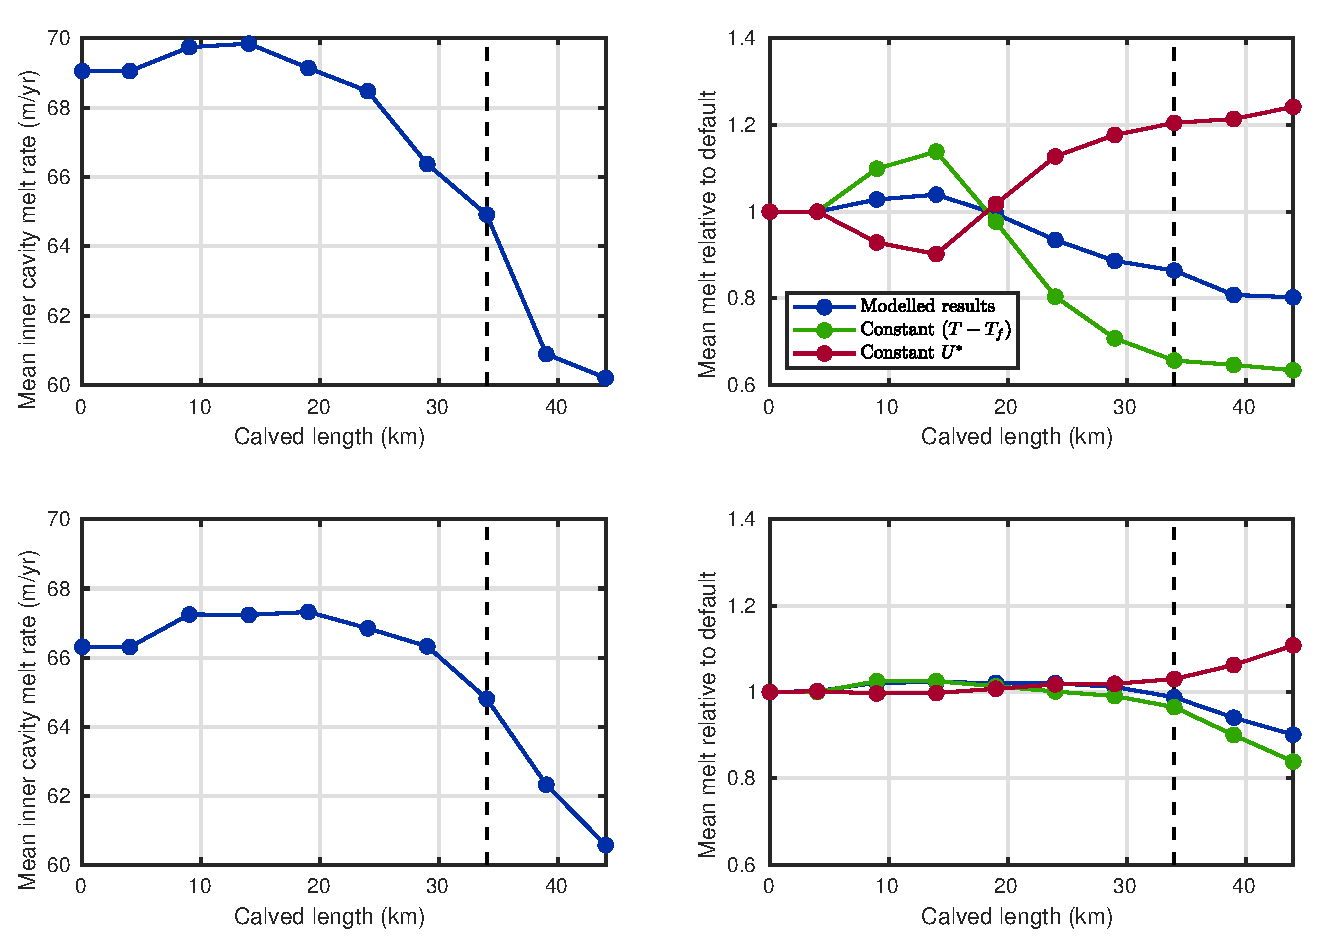
\includegraphics[width = \textwidth]{../make_figures/plots/figure6.eps}
    \caption{(a) Inner cavity melt rate as a function of the calved length $l_c$ for $W$=100~m (light grey, as in figure~\ref{fig:figure4}a), $W$=150~m (blue), and $W$=200~m (green). The black dashed line indicates the position of the ice front when it is located directly above the seabed ridge. (b)-(c) Velocity-thermal driving decomposition (i.e. as in figure~\ref{fig:figure4}b) for (b) $W$ = 150~m and (c) $W$ = 200~m.}
    \label{fig:figure6}
\end{figure}

\begin{figure}
    \centering
    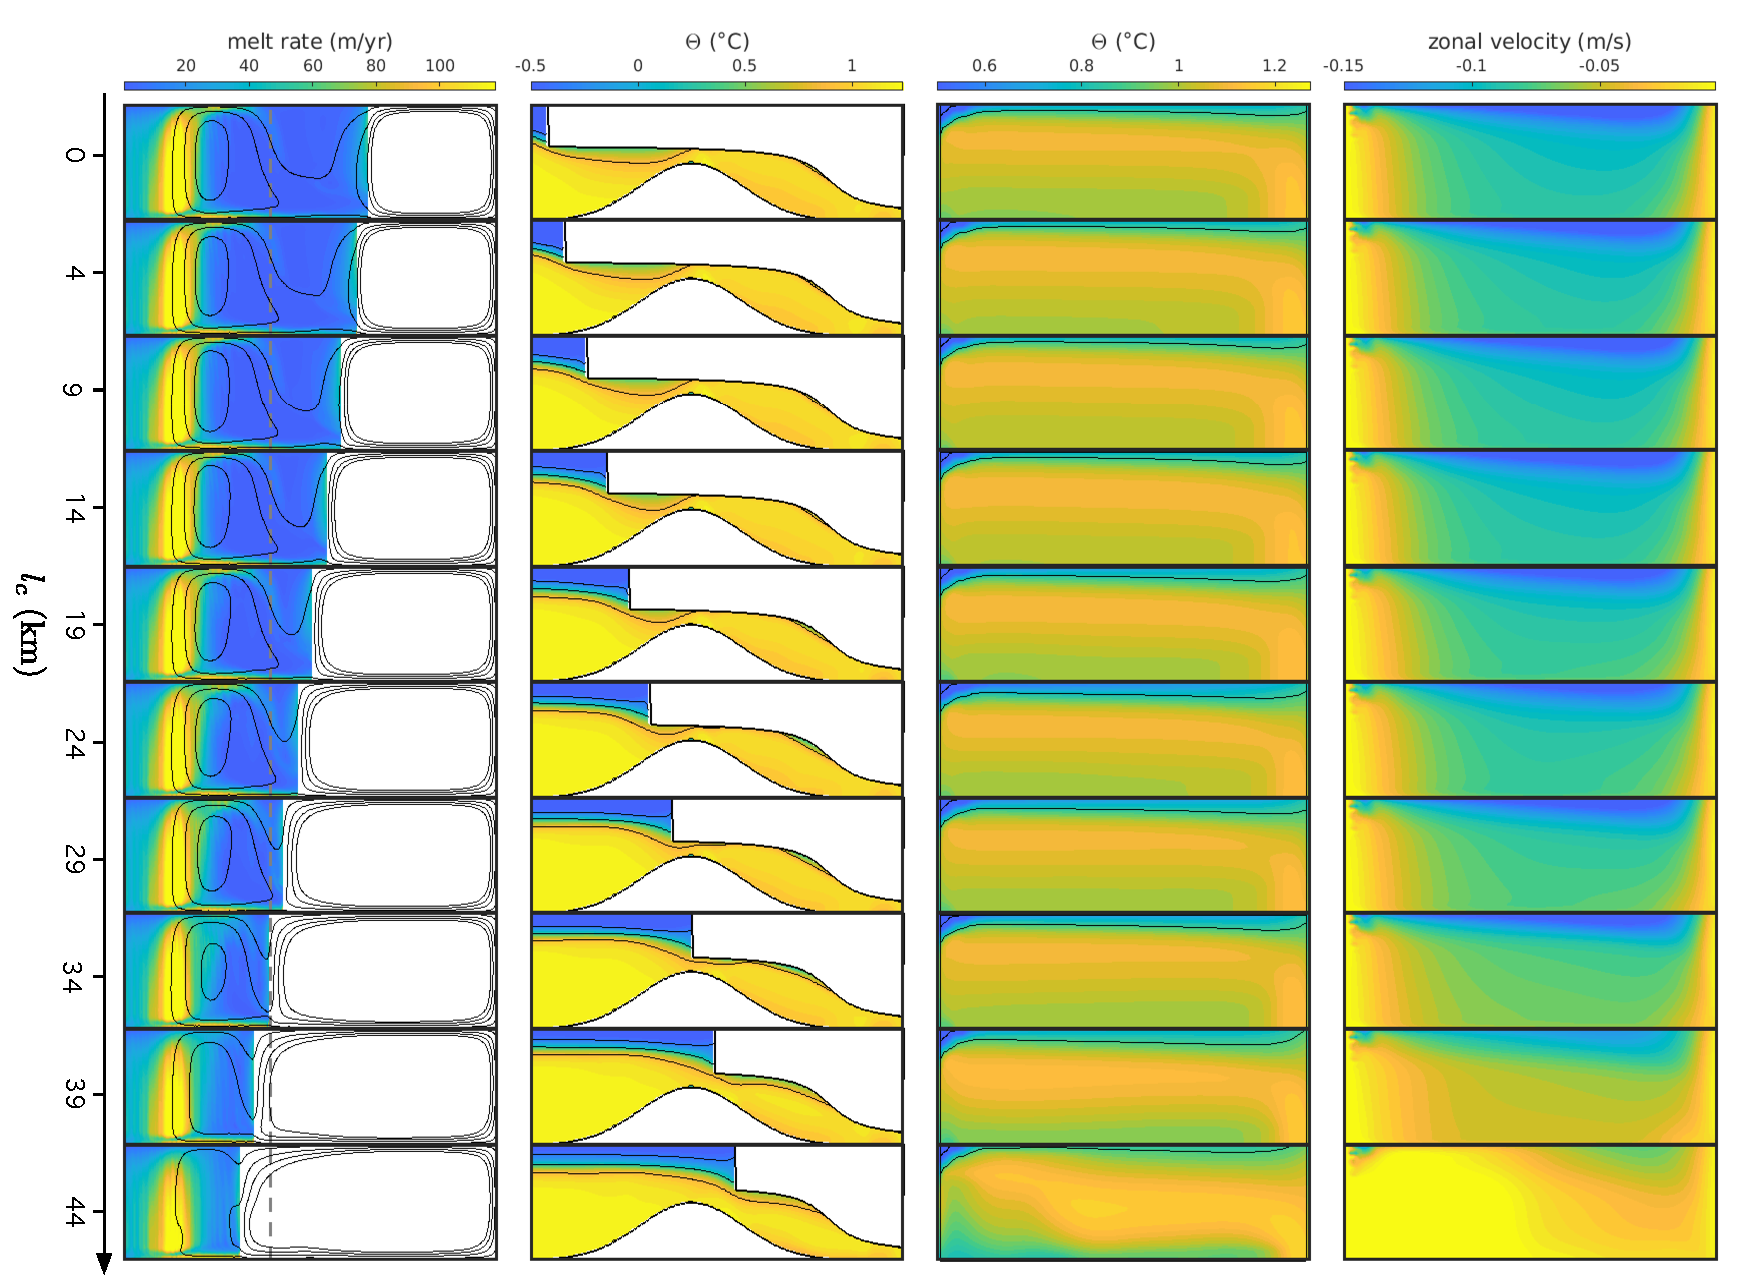
\includegraphics[width = \textwidth]{../make_figures/plots/figure7_axislabel.pdf}
    \caption{Ocean characteristics in the idealized simulation with $P$ = 600~m and $W$ = 200~m. This plot is as in figure~\ref{fig:figure5} for the simulation with $W$=200~m.}
    \label{fig:figure7}
\end{figure}


%what do we see
Mean melt rates as a function of calved length $l_c$ for $W$=150~m and $W$=200~m are plotted in figure~\ref{fig:figure6}a. As in the $W$=100~m case, the inner cavity melt rate reaches a maximum when the ice front is located offshore of the ridge crest. In addition, the velocity-thermal driving decomposition indicates that for both $W$=150~m and $W$=200~m, the reduction in inner cavity melt rates for $l_c$ above the value at which the maximum melt rate is attained results from a reduction in the inner cavity circulation that outweighs an increase in thermal driving. There are, however, two important differences to the $W$=100~m case: firstly, the inner cavity melt rate is far less sensitive to calving for both $W$=150~m and $W$=200~m cases (the difference between largest and smallest inner cavity melt rates is approximately 20\% and 10\%, respectively, compared to 60\% for $W$=100~m). Secondly, these larger gap scenarios do not display a threshold-like behaviour, with the inner cavity melt rate dropping suddenly as the calving front reaches the top of the ridge, as it does in the $W$=100~m case. These observations are consistent with the results of~\citeA{DeRydt2014JGeophysResOceans}, who identified that the melt rates in a similar idealized domain do not care about the ice shelf geometry when the gap between the seabed ridge and ice draft is greater than 200~m.

%why do we see it
\textcolor{red}{To understand these results, it is useful to compare the barotropic streamfunction, and zonal and meridional cross sections that were shown in figure~\ref{fig:figure4} for $W$=100~m to those in figure~\ref{fig:figure7} for the $W$=200~m case (a comparison between the $W$=100~m and $W$=150~m cases is qualitatively similar to that discussed below, but the differences are clearer for $W = 200$m.) Recall that in the $W$=100~m case, the two key mechanisms responsible for the observed melt response to calving are (1) the relaxation of the PV barrier and thus increased connectivity between the cavities inshore and offshore of the ridge, permitting increased warm water access to the inner cavity, and (2) a reduction of the topographic confinement of the cyclonic circulation in the inner cavity. In the $W$=200~m case, the PV barrier is much weaker and the inner and outer cavities are strongly connected, even for the uncalved ($l_c$=0) simulation; there is significant transport of warm water across the ridge (figure~\ref{fig:figure7}a, c, d), and the inner cavity is almost entirely flushed with modified CDW (figure~\ref{fig:figure7}b). This means that ice front retreat, which permits increased warm water access, has only a limited effect. Despite this, we do see that when the ice front is retreated beyond the ridge crest, and any remaining PV barrier provided by the ridge-crest and ice draft is removed, the transport across the ridge increases (figure~\ref{fig:figure7}a,d), the stratification drops (figures~\ref{fig:figure6}c and~\ref{fig:figure7}b) and the melt rate is reduced (figure~\ref{fig:figure6}a).}

\textcolor{blue}{To understand these results, it is useful to compare the barotropic streamfunction, and zonal and meridional cross sections that were shown in figure~\ref{fig:figure4} for $W$=100~m to those in figure~\ref{fig:figure7} for the $W$=200~m case (a comparison between the $W$=100~m and $W$=150~m cases is qualitatively similar to that discussed below, but the differences are clearer for $W = 200$m.) Recall that in the $W$=100~m case, the two key mechanisms responsible for the observed melt response to calving are: (1) the ice front induced vorticity and the relaxation of the PV barrier as the ice front is retreated to the ridge and beyond, which permit a barotropic flow across the ridge, and (2) a reduction of the topographic confinement of the cyclonic circulation in the inner cavity. In the $W$=200~m case, the PV barrier is somewhat weaker than in the $W$=100~m case, and barotropic flow across the ridge occurs, even when the ice front is located offshore of the ridge (figure~\ref{fig:figure7}). As mentioned, this barotropic flow is far more vigorous at flushing the inner cavity than the zero-depth-mean, vertically sheared overturning of that is responsible for flushing in the $W$=100~m case when the ice front is located offshore of the ridge. As a result, the inner cavity is almost entirely flushed with modified CDW (figure~\ref{fig:figure7}b), regardless of the ice front position. Ice front retreat, which permits increased warm water access, has only a limited effect; in particular, this removes the tendency for both increasing temperature and circulation that we see in the $W$=100~m case, before the ice front is retreated to the ridge.}

\textcolor{blue}{Although there is barotropic flow as the ridge for all values of $l_c$, when the ice front is retreated to -- and beyond -- the ridge, the ice front induced vorticity and the relaxation of the PV barrier mean that barotropic flow across the ridge increases further. As a result, the inner cavity stratification reduces (figures~\ref{fig:figure6}c and~\ref{fig:figure7}b) and as does the melt rate (figure~\ref{fig:figure6}a). The increase in barotropic flow is not as acute as in the $W$=100~m case, and  thus the sharp reduction in melt rates is not observed.}



\section{Effect of Hydrographic Conditions on Melt Response to Calving}\label{S:Results:P}
Before moving on to assess how the inner cavity melt rate responds to calving in the realistic simulations, we briefly consider how the picture presented in the previous two sections changes depending on the hydrographic forcing. Since we consider a constant ridge height, variations in the difference between the pycnocline depth and the depth of the ridge crest -- which we expect to be a key driver of the quantity of warm water that is able to spill over the ridge and into the inner cavity -- is captured here by variability in the value of $P$.

\begin{figure}
    \centering
    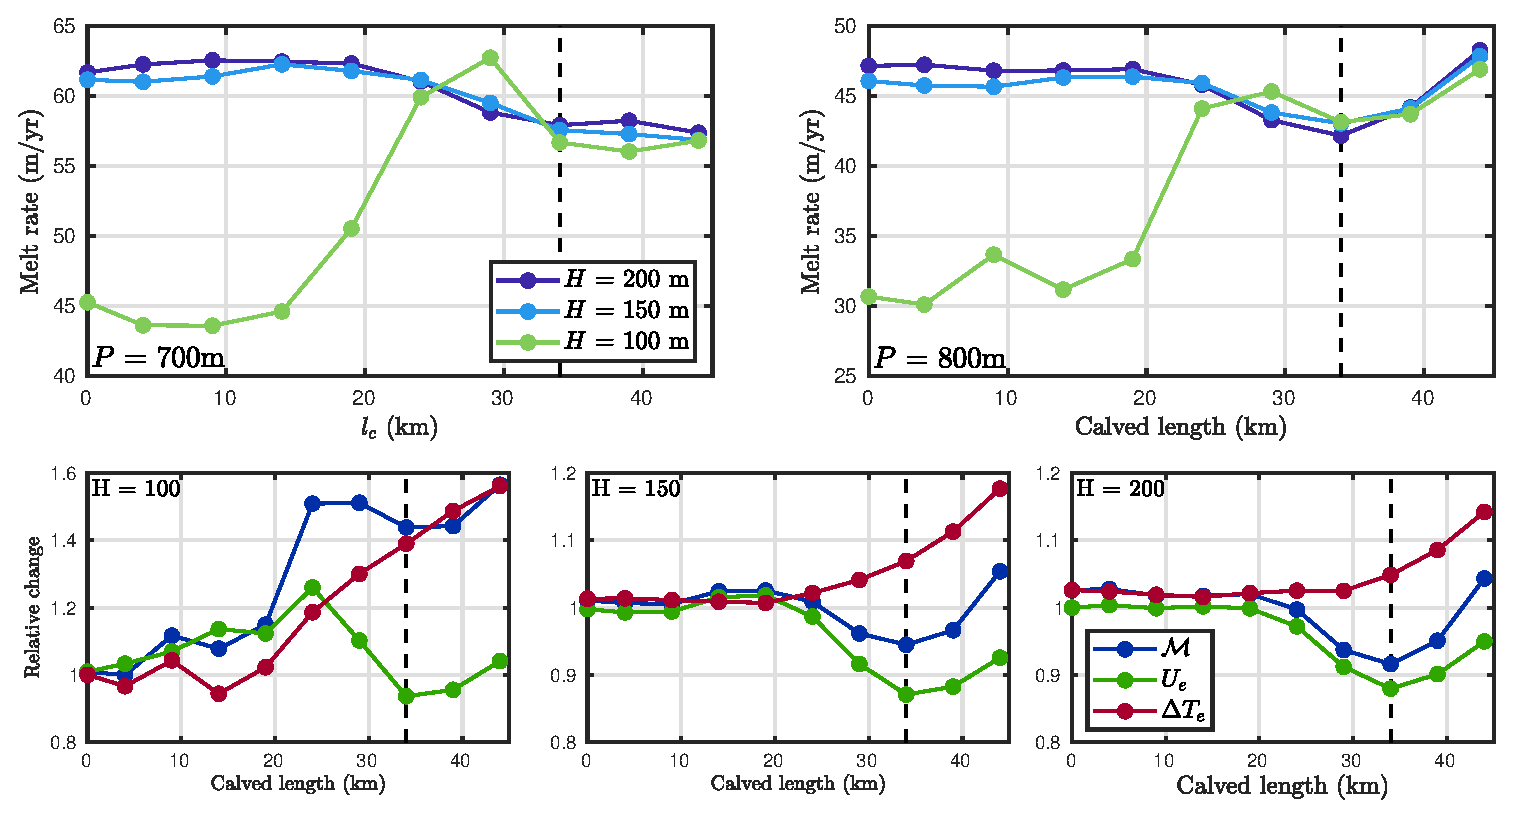
\includegraphics[width = \textwidth]{../make_figures/plots/figure8.eps}
    \caption{(a)--(b) Inner cavity melt rate as a function of calved length $l_c$ in idealized Pine Island simulations with (a) $P$=700~m and (b) $P$=800~m. Colours correspond to different values of $W$, as indicated by the legend in (a). The black dashed line indicates the location of the crest of the sea-bed ridge. (c)--(e) Velocity--thermal driving decompositions (as in figure~\ref{fig:figure4}) for the the data shown in (b): (c), (d), and (e) correspond to the results for $W$=100~m, $W$=150~m, and $W$=200~m, respectively, as indicated.}
    \label{fig:figure8}
\end{figure}


% Introduce simulations with reminder of what they correspond to 
The inner cavity melt rate and velocity-thermal driving decomposition for the three experiments with $P$ = 700~m (hydrographic forcing as in the dashed profiles in figures~\ref{fig:figure2}b and c) and the three experiments with $P$ = 800~m (dot-dashed profiles) are plotted in figure~\ref{fig:figure8}. The results for $P$=700~m are similar to those for $P$=600~m: for the narrowest gap ($W$=100~m), the inner cavity melt rate is sensitive to the front position, increasing rapidly as the ice front is retreated towards the ridge crest, before dropping off sharply when the ice front reaches it, and does not change under further ice front retreat. For the wider gaps ($W$=150~m, $W$=200~m), the melt rates are far less sensitive to changes in ice front position, reaching a peak when the ice front is located some way offshore of the ridge (figure~\ref{fig:figure8}a) and decreasing steadily with further ice front retreat beyond this point. A velocity-thermal driving decomposition for the experiments with $P$=700~m (not shown) is qualitatively similar to the $P$=600~m case discussed above:  these results can be explained by the interaction between changes in the amount of heat that is able to reach the inner cavity and topographic confinement of the cyclonic circulation there. The similarity between the $P$=600~m and $P$=700~m cases is perhaps unsurprising when framed in terms of the relationship between the depths of the pycnocline and the ridge crest: in both cases, the CDW layer extends all the way to the top of the ridge (see figure~\ref{fig:figure2}) and thus the seabed ridge alone does not provide a significant barrier to CDW access to the inner cavity.

%results are different for P = 800 -- how?
In the $P$=800~m case, the melt rate is either constant or increases as the ice front is retreated while it is located offshore of the ridge, depending on the value of $W$ (figure~\ref{fig:figure8}b). A reduction in the boundary layer velocity is responsible for a drop in inner cavity melt rates as the ice front is retreated towards the ridge crest (figure~\ref{fig:figure8}c--e), as in the $P$=700~m and $P$=600~m cases. This $P$=800~m case differs from the $P$=600~m and $P$=700~m cases, however, in that subsequent calving taking the ice front beyond the ridge results in an \emph{increase} in the inner cavity melt rate (figure~\ref{fig:figure8}b), which is associated with a reversal of the reduction in boundary layer velocity (figure~\ref{fig:figure8}c--e) (i.e. the boundary layer velocity effect increases when the ice front is retreated beyond the ridge). The important difference in this case that the seabed ridge alone is able to provide a significant barrier, preventing warm water from reaching the inner cavity since the CDW layer in the outer cavity does not extend to the top of the ridge (figure~\ref{fig:figure9}). Therefore, the inner cavity is not flooded with CDW after the ice front is retreated to sit above the ridge crest, unlike in the simulations with smaller values of $P$. Subsequent ice front retreat increases the stratification further, leading to a strengthening of the circulation, which works in tandem with increased heat content to increase the inner cavity melt rate.


\begin{figure}
    \centering
    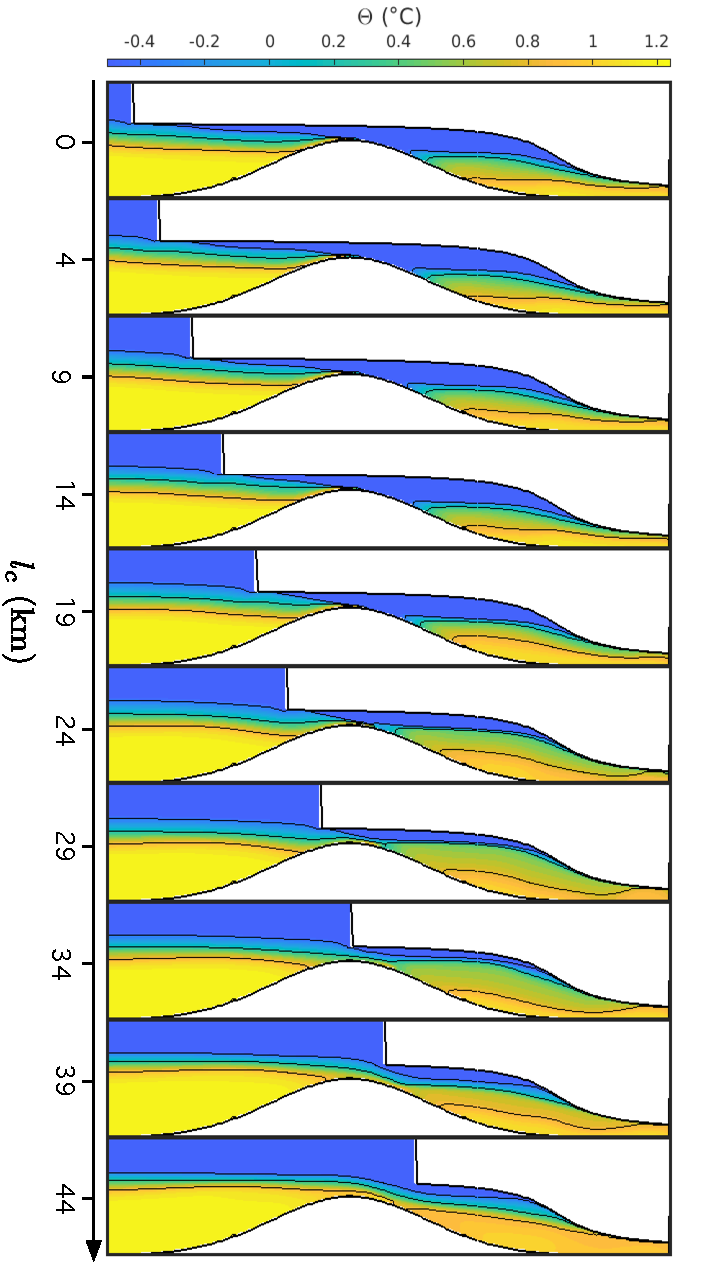
\includegraphics[width = 0.35\textwidth]{../make_figures/plots/figure9_axislabel.pdf}
    \caption{Meridional cross sections for simulations with $P$=800~m, $W$ = 100~m. This plot is as in figure~\ref{fig:figure5}b for the simulation with $P$=800~m, $W$ = 100~m. }
    \label{fig:figure9}
\end{figure}

\section{Assessing the Melting Response of PIIS to Calving}\label{S:Realistic}
% intro to the section
The experiments described in \S\ref{S:Experiment}--\S\ref{S:Results:P} reveal how melt rates near the grounding line in an idealized geometries with a uniform ridge-draft gap may respond sensitively to calving, depending on the geometry of the cavity and, in particular, the gap between the ice draft and seabed ridge. These idealized experiments inform our understanding of a similar experiment that is designed to assess the response of melt rates on PIIS calving. In this section, we describe this experiment, and present and analyze the results.

\begin{figure}
    \centering
    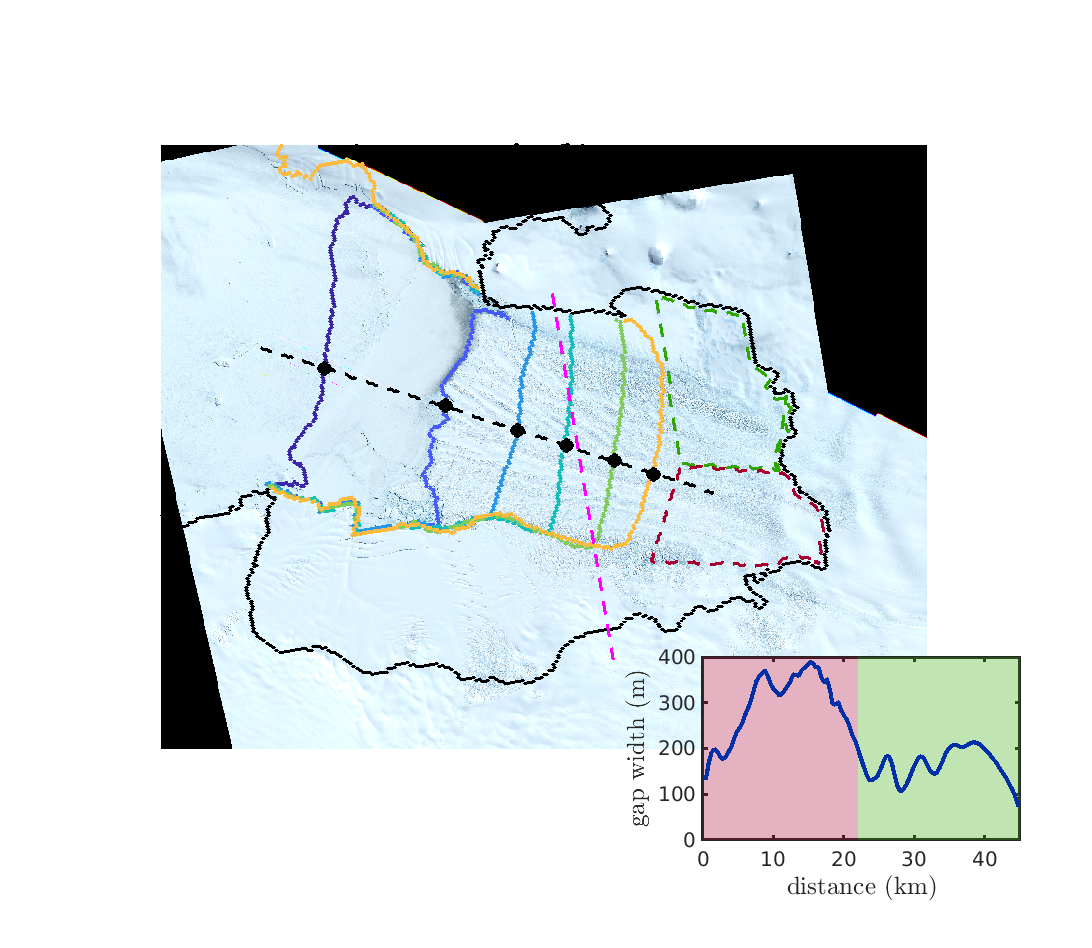
\includegraphics[width = 0.75\textwidth]{../make_figures/plots/figure10.eps}
    \caption{Ice front positions used in simulations to assess the response of melt rates on PIIS to calving. Each simulation corresponds to a different ice front position, indicated by the curves in the purple to yellow colormap curves; dark purple and blue ice fronts correspond to the 2009 and 2020 front positions, respectively (as indicated). The solid black line indicates the location of the 2009 grounding line from~\citeA{Joughin2010GRL}. The blue dashed line roughly indicates the centreline of the cavity, along which the calved length -- the difference between the ice front and the 2009 ice front -- is measured, and the black dashed line approximately indicates the peak of the seabed ridge. The cyan (North) and magenta (South) boxes indicate the inner cavity regions considered in the experiments (see main text). Inset: plot of the (vertical) gap between the ridge crest and the ice draft, measured along the black dashed line in the main figure. Cyan and magenta shaded sections correspond to locations North and South of the blue dashed centreline, respectively. The background image is a Sentinel 2 mosaic from November 2020.}
    \label{fig:figure10}
\end{figure}

%Describe experiments
\subsection{Experiment Details}
To assess the response of sub-shelf melt rates to calving in Pine Island Glacier, we resolve the circulation in a cavity whose geometry closely resembles PIG (see below). We use the same ocean model as described in \S\ref{S:Experiment:Model} with six different ice shelf topographies. The locations of these ice fronts are shown in figure~\ref{fig:figure10}: the first simulation (purple ice front in figure~\ref{fig:figure10}) uses an ice shelf cavity that corresponds to PIIS in 2009. The second simulation (blue ice front in figure~\ref{fig:figure10}) uses the 2009 ice shelf draft, with a section of ice removed at the front so that the ice front matches the observed ice front position in 2020. The four further simulations similarly use the 2009 ice shelf draft with sections of fast flowing ice (i.e. within the shear margins) removed. We stress that the ice thickness, and thus grounding line position and ice shelf draft, at existing shelf locations remains the same in each simulation: only the ice front position varies between simulations and the ice thickness is not updated, as was the case in the idealized simulations.  %Consistently with the idealized simulations, we refer to the simulation with the 2009 ice front as the default run.

%how do we get cavity and draft
The sub shelf cavity geometry we use computed from the ice and seabed geometry, as described by~\citeA{Dutrieux2014Science}. Briefly, the ice shelf geometry is calculated from a 40~m-resolution digital elevation model (DEM) of the ice freeboard from 2008~\cite{Korona2009Photogrammetry}, that is adjusted with a constant medium bias from observations obtained from the Autosub underwater autonomous vehicle~\cite{Jenkins2010NatureGeo}. The DEM assumes freely floating ice throughout the shelf, which may reduce its accuracy close to the grounding line. Over the continental shelf, the seabed geometry is well known from ship echo-sounding \cite{Dutrieux2014Science}, while in the cavity it calculated from an inversion of gravimetry data and corrected point-wise using the median difference between the depth from the gravimetry inversion and the Autosub observations. 

%model notes and calibration
We consider a single hydrographic forcing, corresponding to observed 2009 conditions in Pine Island Bay (dark grey line in figure~\ref{fig:figure2}b,c), to which the ocean is restored far from the ice shelf. All model parameters are as described in \S\ref{S:Experiment:Model}. In particular, we take the drag coefficient in the three equation formulation of melting to be 4.5$\times10^{-3}$; this value is tuned so that the total meltwater flux in the simulation with the 2009 geometry (86 Gt yr\textsuperscript{-1}) closely matches the estimated total meltwater flux for 2009 (80 km\textsuperscript{3}/yr) \cite{Dutrieux2014Science}). % The simulated melt rate for the `uncalved' simulation with the 2009 ice shelf geometry (figure~\ref{fig:figure11}a) is consistent with observations (not shown), displaying complex features on small scales, but characterized on larger scales as being concentrated near to the grounding line, with a peak melt rate of approximately 120~m~yr\textsuperscript{-1}.

%gap is not uniform, but sort of split. Tell the reader what the different regions are.
As mentioned in \S\ref{S:Experiment:Model} the ridge-draft gap under PIIS is not uniform but varies from 100~m at its narrowest to 400~m at its widest. (This motivated the choice of gap thicknesses $W$ in the idealized simulations of \S2--5.) The ridge-draft gap (inset in figure~\ref{fig:figure10}) can be approximately partitioned into two sections: in the Southern part of the inner cavity (magenta shading on inset of figure~\ref{fig:figure10}), the gap is relatively wide, while in the Northern part of the inner cavity (cyan shading) the gap is narrow; to facilitate inferences from our idealized results -- which consider a uniform ridge-draft gap -- to be made, we evaluate changes in melting with calving in two separate regions inshore of the ridge, whose boundary corresponds to the upstream extrapolation of the boundary between the narrow and wide sections of the ridge-draft gap (see figure~\ref{fig:figure10}). 

\subsection{Results}

\begin{figure}
    \centering
    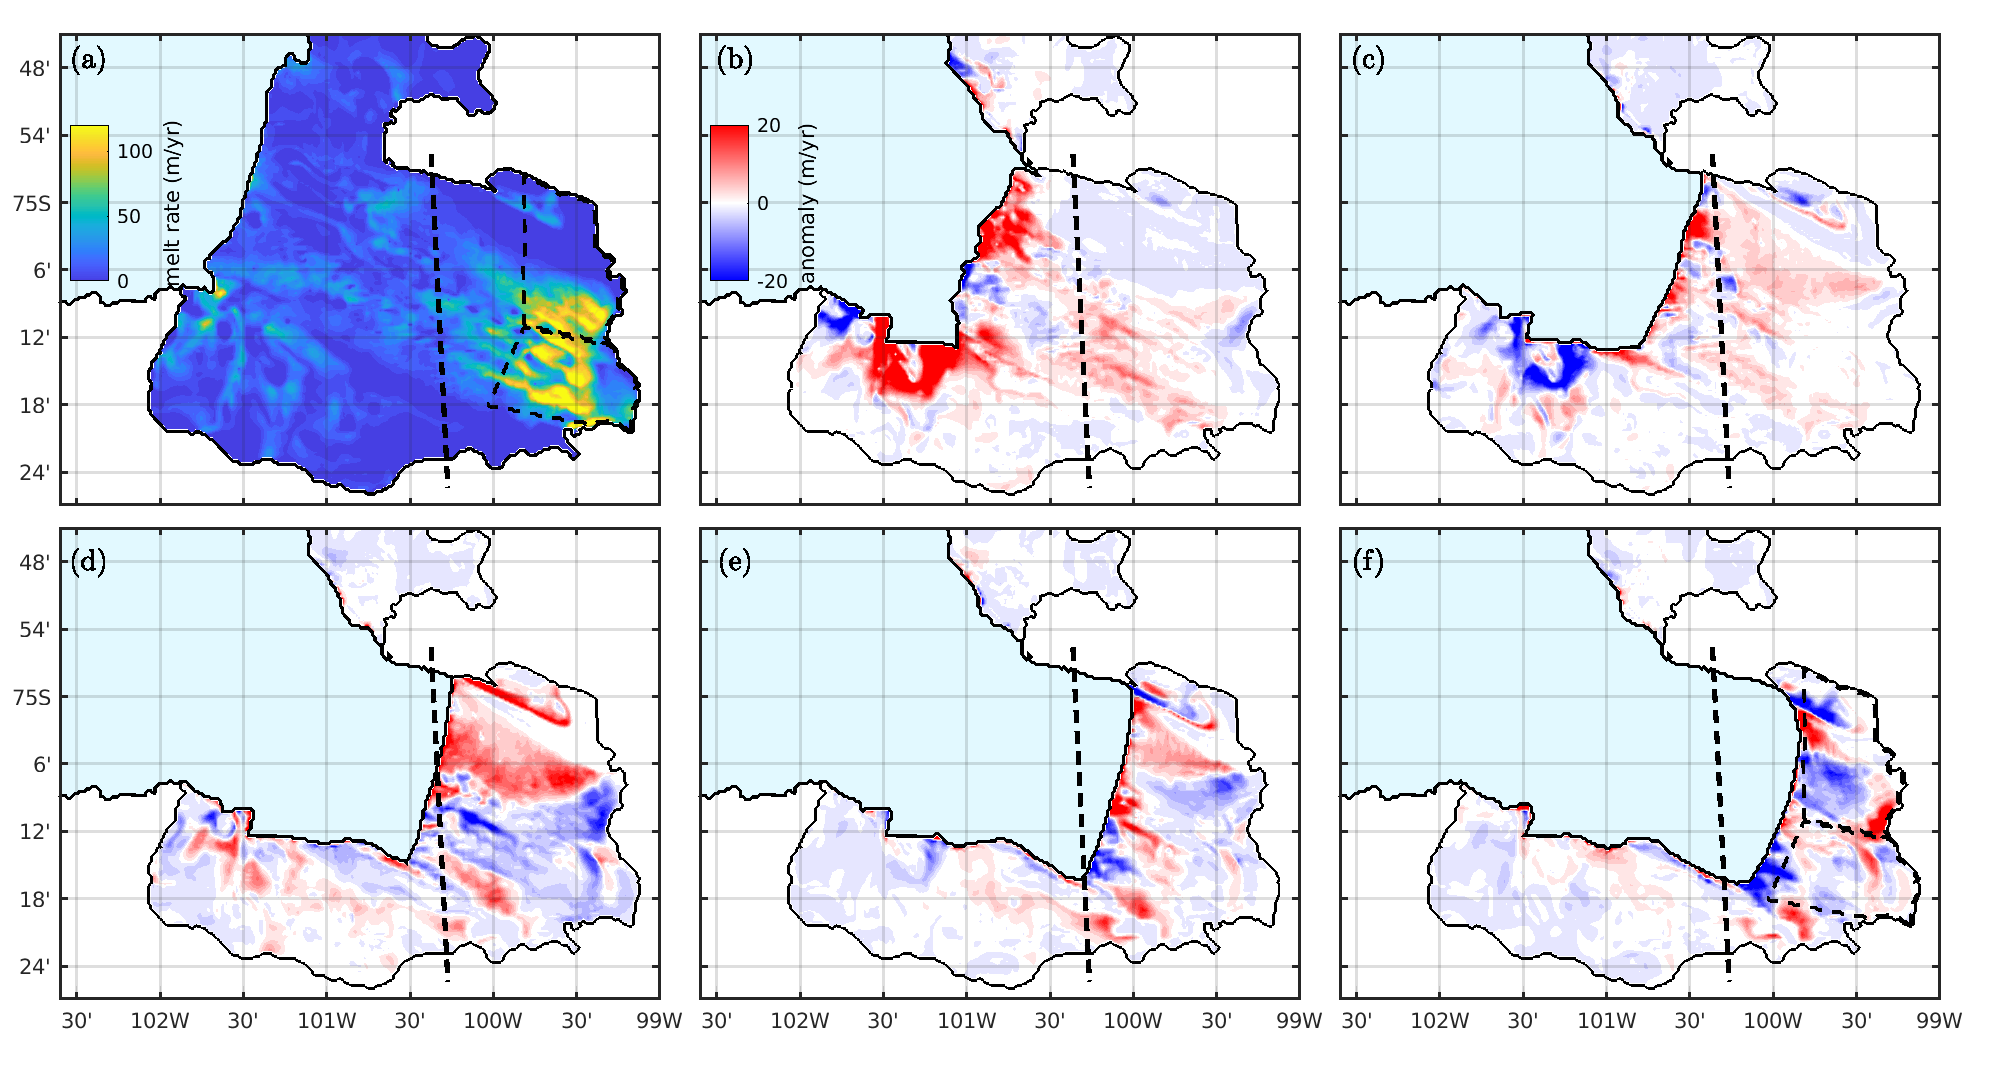
\includegraphics[width = \textwidth]{../make_figures/plots/figure11_labelled.pdf}
    \caption{(a) Simulated melt rate in the 2009 Pine Island geometry. Black dashed boxes (also in (f)) indicate the North and South boxes (see figure~\ref{fig:figure10}), where the highest melt rates are concentrated. (b)--(f) Non-cumulative melt rate anomaly in the simulations (i.e. measured relative to the previous panel). The colourbar in (b) is appropriate for each of (b)--(f). In each case, ice shelf front and grounding line (2009 grounding line position from ~\cite{Joughin2010GRL}) are shown as a solid black line, and the approximate location of the ridge crest as a black dashed line.} 
    \label{fig:figure11}
\end{figure}


%introduce simulations
Figure~\ref{fig:figure11} contains a plot of the simulated melt rate in the 2009 geometry, as well as non-cumulative melt rate anomalies for the other five simulations in the experiment. To be explicit, non-cumulative here means that red (blue, respectively) locations on these maps indicate areas in which the melt rate increases (decreases) when the ice front is retreated from its position as the next largest ice shelf, i.e. changes in melt are shown relative to the previous simulation in the series, rather than relative to the first (2009) simulation.

%Melt rates look qualitatively similar in the default run to the idealized case
The pattern of melt rates in the 2009 simulation (figure~\ref{fig:figure11}a) is qualitatively similar to the corresponding uncalved ($l_c$ = 0~km) idealized simulation (figure~\ref{fig:figure5}a): peak melt rates are concentrated near to the grounding line, reaching a peak of approximately 120~m yr\textsuperscript{-1} several kilometers downstream of it, while the melt rate in the majority of the shelf is below 20~\mpryr. This pattern of simulated melt rates under PIIS is consistent with observations~\cite{Dutrieux2014Science} and other numerical simulations of cavity circulation under PIIS~\cite{Heimbach2012AnnGlac}.

%2009--now: large anomalies at the front
When the ice front is retreated from its 2009 position to its 2020 position, melt rates within 10~km of the ice front increase significantly (figure~\ref{fig:figure11}b). This is attributed to high velocities associated with upwelling at the new ice shelf front as well as the formation of a gyre in the exposed open ocean, which is covered by the ice shelf in the 2009 simulation, as has been observed in practice~\cite{Yoon2021}. The gyre results in a strong circulation along the ice shelf front, which acts a dynamic barrier to flow as well as providing a freshwater source to further enhance the flow. Melt rates in the inner cavity do not change significantly, when the ice front is retreated from its 2009 position to its 2020 position: the average melt rate in the Northern and Southern boxes increases by approximately 1\mpryr and 2\mpryr respectively (figure~\ref{fig:figure12}a).

%Qualitative descriptions of melt anomalies: (a) characterized by complex patterns, (b) only see significant changes when calving beyond the ridge (large positive anomaly in the northern shear margin which might be important for stability), (d) melt rates decrease when ice front has retreated significantly (this is a lead in to the qualitative analysis of fig 12)
Melt rate in the simulations with possible future ice front positions display complex patterns of change, featuring large regions of both positive and negative anomalies (figure~\ref{fig:figure11}). We highlight several important features of these patterns: firstly, melt rates does not change significantly in the first 'future' scenario, suggesting that PIIS currently has a reasonable `safety band' for changes in melt rate with calving: melt rates are not expected to change significantly until the ice shelf front has retreated some way ($>$10~km) from it current position. Secondly, melt rates in the vicinity of the Northern shear margin increase dramatically when the ice front is retreated to a position that sits (approximately) above the seabed ridge (figure~\ref{fig:figure11}d), and this region of enhanced melt rates extends almost all the way to the grounding line.  Finally, melt rates decrease significantly over large portions of the areas of the ice shelf once the front has retreated a significant distance upstream of the ridge (figure~\ref{fig:figure11}f).

\begin{figure}
    \centering
    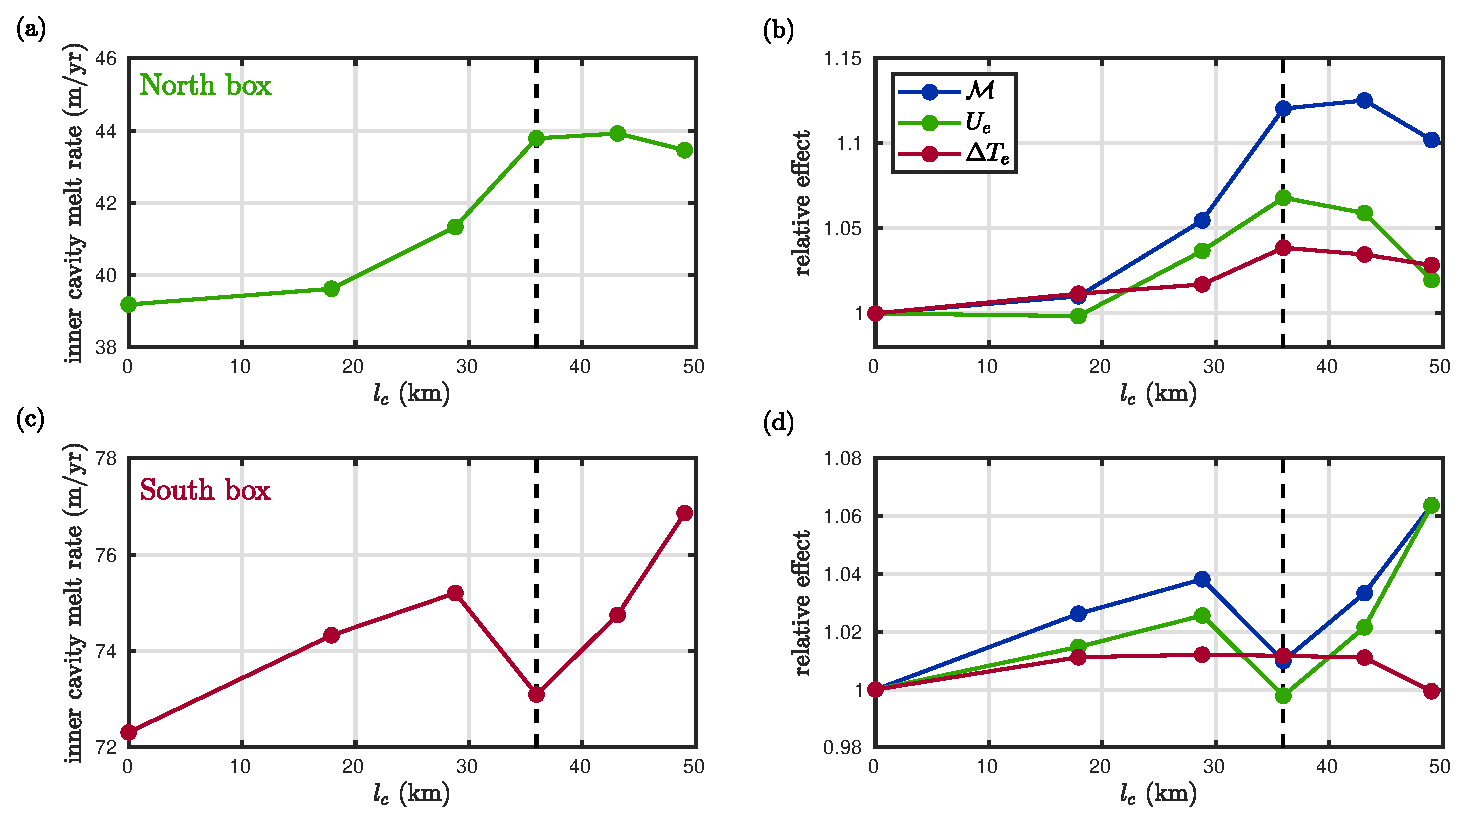
\includegraphics[width = \textwidth]{../make_figures/plots/figure12.eps}
    \caption{(a), (c) Average melt rate as a function of calved length $l_c$ in simulations using a cavity geometry that closely resembles Pine Island. Plots (a) and (c) correspond to the North and South regions of the inner cavity, which are shown in figure~\ref{fig:figure10} as cyan and magenta dashed boxes, respectively. The calved length $l_c$ is the distance measured along the blue dashed line in figure~\ref{fig:figure10}, taken relative to the 2009 ice front position (purple curve in figure~\ref{fig:figure10}.). (b), (d) Velocity-thermal driving decomposition for the changes in melt rate shown in (a) and (c), respectively. As indicated by the legend in (b) and (d), blue, red, and green curves correspond to simulated changes $\mathcal{M}$, velocity effects $U_e$, and thermal driving effects $\Delta T_e$, respectively. In each of  plots, the black dashed line approximately corresponds to the calved length when the ice front sits approximately above the ridge crest (this is the distance from the intersection of the blue and black dashed lines in figure~\ref{fig:figure10} to the 2009 ice front, measured along the blue dashed line.}\label{fig:figure12}
\end{figure}

%these qualitative observations sort of agree with the mean melt rate plots
 These observations are in qualitative agreement with the idealized simulations presented in \S2--5. To go beyond this qualitative assessment, we plot in figure~\ref{fig:figure12}, the mean melt rate as a function of calved length for each of the two boxes introduced earlier. In the Northern box, mean melt rates remain approximately constant until the ice front approaches the seabed ridge, where they increase sharply, before seeing a weak reduction as the ice front is retreated further. In the Southern box, melt rates are less variable (in terms of \% change), but the overall trend is that the melt rate increases while the ice front is located downstream of the seabed ridge, before dropping temporarily when the ice front is retreated to the ridge and subsequently increasing again. 
 
%northern box 'hides' behind a narrow gap -- make comparison with the narrow idealized case
Our interpretation of these results is guided by the idealized simulations presented in \S\ref{S:Baseline}--\ref{S:Results:P}. The Northern box, the inner cavity `hides behind' a relatively narrow gap between the seabed ridge and the ice draft (figure~\ref{fig:figure10}), and the change in melt rates with calving behaves in a qualitatively similar way to idealized results with narrow ($W$=100~m, $W$=150~m) gaps. A velocity-thermal decomposition of these changes in melt rates indicates that -- as in the corresponding idealized case -- both increases in thermal driving and velocity contribute to the increases in melt rate with calving while the ice front is located offshore of the ridge, and that a reduction in the boundary layer velocity is responsible for the decrease in melt rates when the ice front is retreated beyond the ridge. By drawing analogy with the idealized simulations, we assert that the enhancement in melt rates with calving while the ice front is located offshore of the ridge is driven by increased heat reaching the inner cavity via boundary currents and an enhanced circulation within the inner cavity that results from the associated increase in stratification, while the reduction in melt rates when the ice front is retreated to the ridge results from a relaxation of the confinement of the cyclonic circulation in the inner cavity and a reduction in stratification as the inner cavity that results from a flooding of the inner cavity with warm water.

%In the idealized case, however, the effect of a reduction in the boundary layer velocity was stronger, and the decrease in melt rate larger, than in this realistic case; we attribute this difference to the splitting of a connected domain into two sub-regions, and the particular complexities of the realistic cavity.

%southern box 'hides' behind a wide gap -- make comparison with the wide idealized case
The Southern box `hides behind' a relatively wide gap between the seabed ridge and the ice draft (figure~\ref{fig:figure10}). As was the case for idealized simulations with wide ($W \gtreq$200~m), the mean melt rate is largely insensitive to the ice front position than it is with a narrow gap (i.e for the Northern box): the difference between the minimum and maximum melt rates in the Southern box is approximately 6\%, which is almost half of the corresponding value in the Northern box. The overall trend of increasing melt rates except for a drop when the ice front is located on top of the ridge associated with a reduction in velocities (figure~\ref{fig:figure12}) is reminiscent of the results of the idealized simulations with a lower pycnocline (see figure~\ref{fig:figure8}(b)--(e)); drawing analogy to the idealized results, this suggests that the Southern cavity is not entirely flooded with warm water, and ice front retreat continues to increase stratification, even after the ice front has been retreated beyond the ridge.


\begin{figure}
    \centering
    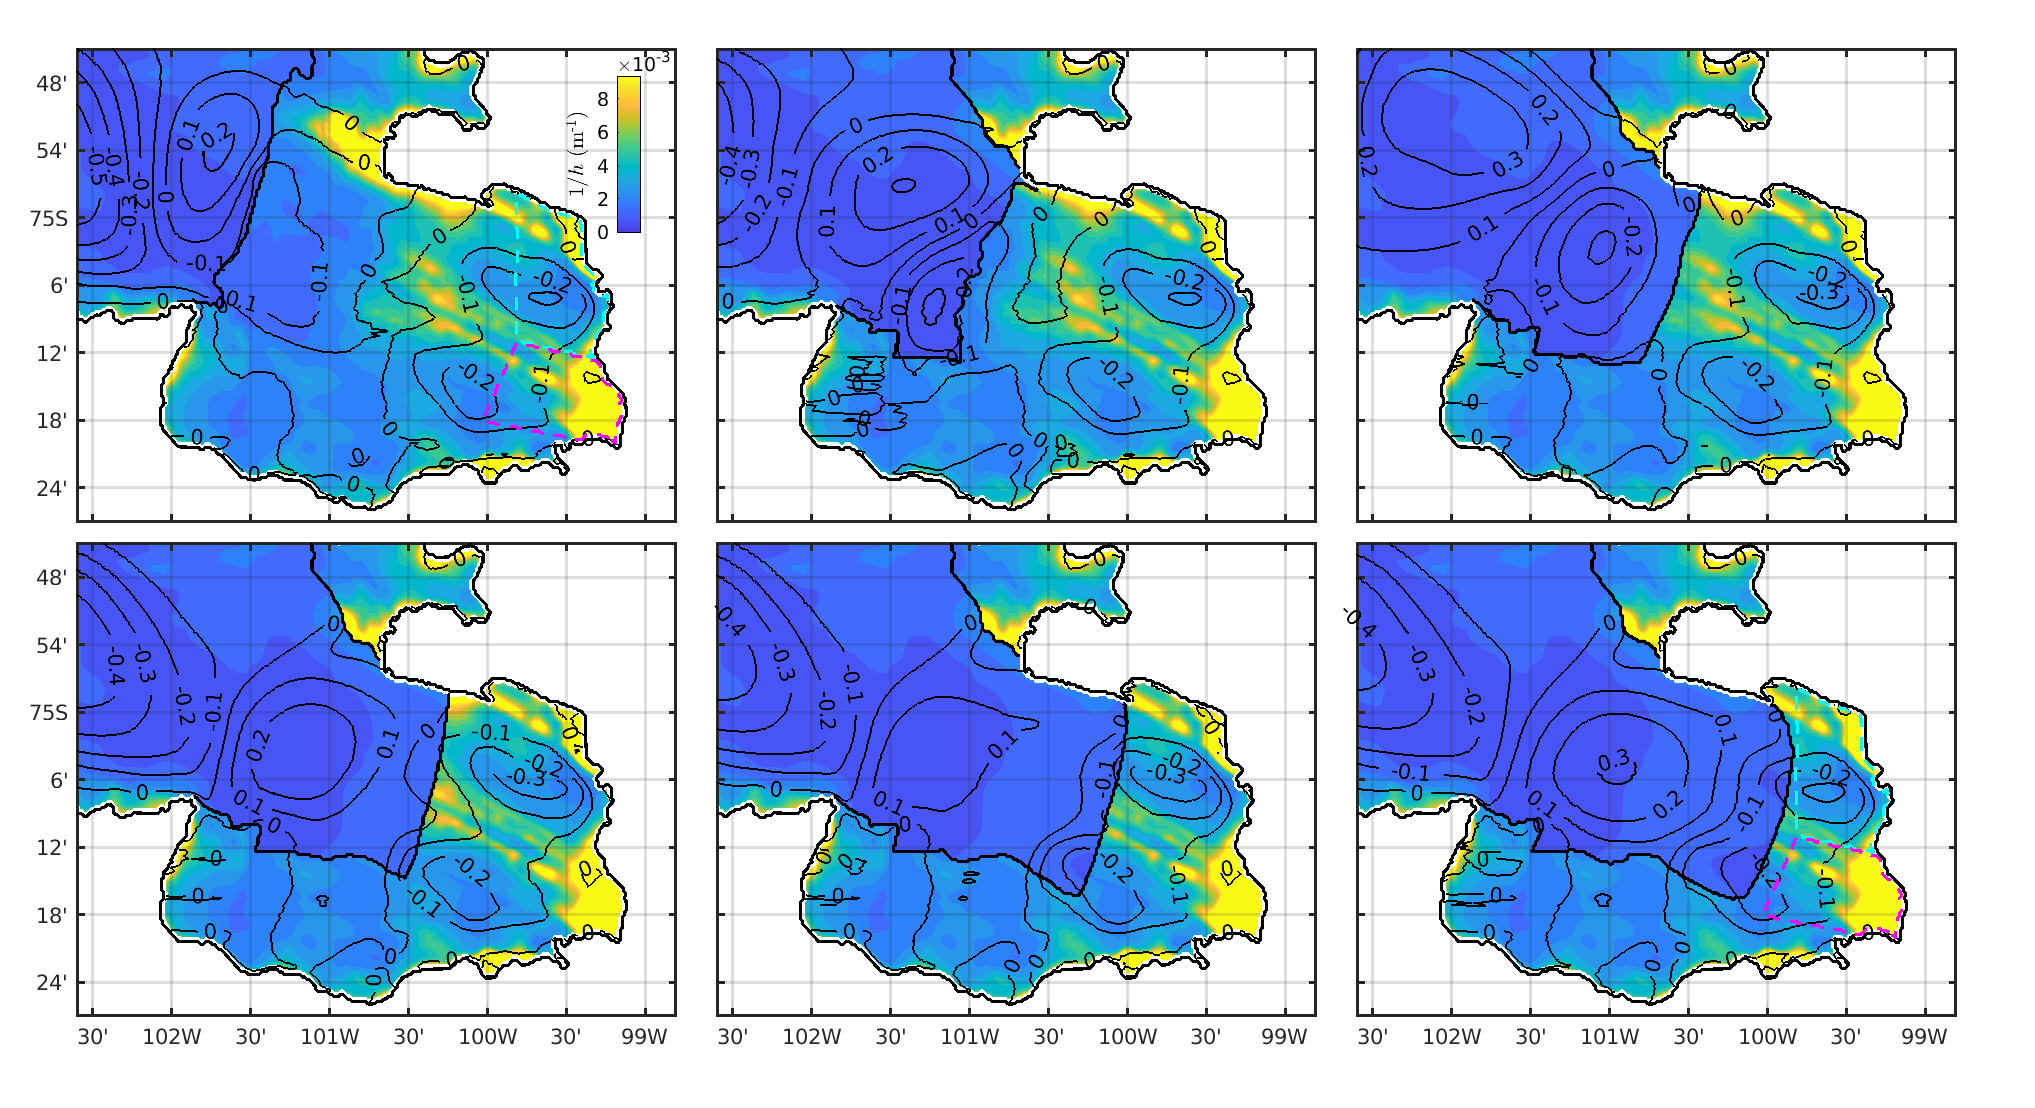
\includegraphics[width = \textwidth]{../make_figures/plots/figure13.eps}
    \caption{\red{to be completed. Plots of BSF. Relevance to text: (1) shows formation of the gyre at the ice front, (2) offers some justification that the two regions of the inner cavity are `separable'}} 
    \label{fig:figure11}
\end{figure}
\section{Discussion}\label{S:Discussion}

%haven't yet seen big anomalies in melt rates at the gl --> suggests that buttressing changes driven by calving, not melting. Need coupled model to probe interaction between them
For the immediate future of PIIS, the salient observation from the realistic simulations presented in the previous section is that the inner cavity melt rates do not change significantly when the ice front is receded from its 2009 position to its 2020 position. This suggests that changes in melting associated with relaxation of the topographic barrier under PIIS have yet to occur. The reduction in buttressing that resulted in the recent acceleration of PIG \cite{Joughin2021ScienceAdv} must derive primarily from  the loss of ice shelf area, rather than thinning of the ice shelf near the grounding line driven by changes in melting that followed (the region around the grounding line is particularly important for buttressing~\cite{Reese2018NatureClimCh}). On longer timescales, these two processes are coupled; investigating their relationship requires the use of a coupled-ice ocean model, which is beyond the scope of this paper. (Here, we concerned ourselves only with the immediate melt response to calving, rather than the subsequent ice dynamic response.)

%use this nice lead in to talk about shortcomings from not updating the cavity thickness 
However, our lack of ice dynamics considerations remains a limitation. In particular, with the exception of the removing sections of the ice shelf, the ice shelf cavity and grounding line position remain identical between simulations: the geometry of ice shelf cavity is not updated to account for the dynamic ice response to calving. In practice, the recent (2015--2020) acceleration of PIG, with increases in speed of $>$10\% over large sections of the ice shelf and grounded ice, will lead to ice shelf thinning and thus grounding line retreat, directly impacting the cavity geometry. Similarly, we expect that future calving events will reduce ice shelf buttressing, and thus similarly encourage grounding line retreat and cavity geometry changes. 

%Despite little change in inner cavity, have a large anomaly at front
Our simulations suggest that melt rates in a region the region close ($<$10~km) to the ice front have experienced a significant increase as a result of the recent calving of PIIS. These enhanced melt rates will lead to significant local thinning, which may encourage further calving events since the critical cliff height for collapse is thought to be strongly dependent function on the height of the cliff~\cite[ for example]{Crawford2021NatureComms}. In summary, while the melt response to recent calving of PIIS might not have an immediate impact on the ice dynamics, we suggest that it will promote further calving and thus loss of buttressing.

%In future melt rates generally increase in future, but changes are smaller than idealized results suggest (why?)
Very broadly, our simulations suggests that further calving of PIIS will lead to enhanced melting in the Northern part of the inner cavity, and to a lesser extent, the Southern part of the inner cavity. The magnitude of changes in melting with calving were similar to what was expected from the idealized simulations for the Southern section of the cavity (i.e. very small), for which the offshore ridge-seabed gap is wide. For the Northern section of the cavity (narrow ridge-seabed gap), the magnitude of changes is smaller than our idealized simulations predict. We attribute this difference to the complexities of the ice draft and seabed in the realistic simulations, and our somewhat ad hoc splitting of the inner cavity into two subsections. The ridge height is highly anisotropic along its length; our decoupling of the cavity into two sections in a simple attempt to account for this aniostropy, but in practice the two inner cavity regions are closely connected dynamically. Further work is required to understand the role of ridge anistotropy in controlling warm water access to the inner cavity.

%We also see large anomalies in the norther shear margin, which might be worrying
The large melt rate anomalies that are seen when the calving front is retreated to the top of the ridge may have a significant impact on the future behaviour of PIG. The shear margins of PIIS play an important role in buttressing the grounded ice~\cite{Lhermitte2020PNAS}; enhanced thinning of these regions may reduce buttressing and thus increase losses from the grounded ice. If calving events maintain their pace since 2015, this situation will be realized in the mid 2020s. Again, we do not attempt to make quantitative statements on the ice dynamics response to melt induced shear-margin thinning, which requires the use of a coupled ice-ocean model.

%although melt responses are not massive there is uncertainty in the ridge-gap, which might be actual response is larger
The magnitude of changes in inner cavity melt rate are not as large in the realistic simulations as in the idealized simulations. However, there is some uncertainity in both the geometry of the seabed and the ice draft in the realistic geometry; the sensitivity to the ridge-draft gap (via the parameter $W$) that was identified in the idealized simulations suggests that, if, in practice, the ridge-draft gap is marginally smaller than used in our realistic simulation, the melt response to calving might be significantly larger. In addition, the ice draft is not static but varies dynamically; advection of thicker (thinner, respectively) sections of the ice shelf to the ridge crest will narrow (widen) the ridge-draft gap and thus increase (decrease) the sensitivity of melt rates to calving.

%what do results mean for melt rate parametrizations 
The results presented in this paper have implications for melt rate parametrizations. At present, no melt rate parametrization is able to account for the position of the ice front when computing the melt rate~\cite{AsayDavis2017CurrClimChRep}; in this paper, we have demonstrated that the ice front position can be an important control on the melt rate applied to an ice shelf. This provides motivation for improvements in melt rate parametrizations. % Although the seabed ridge under PIIS is rather unique amongst ice shelves, it is one of the fastest changing and largest contributors to current ice loss front Antarctica; accurate future projections of PIG are       and thus most commonly simulated ice shelves. Often melt rate parametrizations are used in these simulations; our results suggest that current melt rate parametrizations must be enhanced to account for the seabed ridge if they are to be trusted in projections of PIIS.

%another source of uncertainty are parameter choices in the model, but they don't affect conclusions.
Finally, we note that MITgcm has a plethora of parameter choices and numerical settings, which might have an impact on the results of the simulations. These include choices of grid resolution, which are 400~m in the horizontal (to ensure mesoscale eddies are well resolved) and 10~m in the vertical. Simulations at higher vertical resolution (5~m) did not change the results significantly, although results were somewhat different for lower resolution (20~m); this is perhaps unsurprising because exchange over the ridge crest, which we have shown to be important in controlling the inner cavity melt rate, is expected to be highly sensitive to vertical resolution. Agreement with the higher resolution simulations (5~m) gives us confidence that the simulations presented here are appropriately resolving exchange processes over the ridge crest. 

\section{Summary}\label{S:Summary}
%general overview of the question and answer
The central aim of this study is to understand how, and why, melt rates on Pine Island Ice Shelf might respond to calving events that have already taken place, and those that might occur in future. We suggested at the outset that such calving events might relax the topographic barrier that currently restricts the access of warm water access to the inner cavity which is inshore of the ridge. We have used numerical simulations in both an idealized domain, and one that is representative of PIIS to answer this question.
%what did we see in the idealized simulations, and stress that they can be used as an archetype for situations in which there is a geometric barrier (e.g. if the ice shelf retreats on an overdeepened bed)
Our idealized geometry experiments were designed to isolate parametric dependence in how the melt rate responds, as well as offer insight into the mechanisms responsible for this response. We identified a sensitive dependence on the cavity geometry via the parameter $W$ that describes the gap between the seabed ridge and the ice draft. For a narrow gap ($W \lesssim$ 150~m) with significantly different behaviour for configurations with narrow ($W<$150~m) and wide ($W$>150~m) gaps. The main results are as follows (1) the inner cavity melt rate does not change significantly with the ice front retreat while the ice front is located someway ($>$20~km) offshore of the ridge, (2) as the ice front is retreated towards the ridge, the inner cavity melt rate increases signficantly, before (3) dropping off sharply when the ice front is retreated to sit on top of the ridge if the pycnocline is relatively high or (4) increasing further if the pycnocline is relatively deep. In contrast, for configurations with wide gaps, the melt rate is largely independent of the location of the ice front. We elucidated the roles of heat access to (and resulting stratification of) the inner cavity, and the topographic confinement of a cyclonic gyre that forms in the inner cavity in these results; in some circumstances, these are complimentary, and in others that are competing. In particular, we saw that increased heat access to the inner cavity may, paradoxically, reduce inner cavity melt rates when it results in reduced stratification and thus a slowing down of the cavity circulation. Although these idealized results are intended to inform our understanding of melt rate changes in Pine Island, they can be considered an archetype for situations in which seabed geometry obscures access of warm water to the grounding line of an ice sheet, a situation that might be realized, for example, in ice sheet retreat over an overdeepended bed. 

%main details on the results of the realistic simulations: complex pattern of changes, large anomaly at the front from 2009-2020 might promote further calving, 
The idealized experiments informed simulations performed using a cavity geometry that closely resembles PIIS, designed to assess how melt rates on PIIS might respond to calving in practice. To account for a significant anisotropy in the ridge-draft gap in this realistic geometry (narrow on one side and wide on the other), we split the `inner-cavity' into two sections, one of which is inshore of the narrow section of the ridge-draft gap, and the other of which is inshore of the wide section of the ridge-draft gap. In the `narrow' cavity, the melt rate increases with calving while the ice front is located offshore of the ridge, before reducing with further calving beyond the ridge, while in the `wide' section, the melt rate is largely independent of calving; both of these observations are consistent with the idealized simulations. By making an analogy with the idealized results, we suggest that the same competing mechanisms of heat access to the inner cavity and topographic confinement of the circulation are responsible.

Our results suggest that PIIS sits in a small safety band: inner cavity melt rates will not change significantly until the ice front retreats closer to the ridge. We stress, however, that this prediction is only based on melt rate response to calving, and does not account changes in ice shelf buttressing associated with the ice lost from a shelf during a calving event. In addition, our realistic simulations suggest that melt rates at the ice front have increased significantly as a result of calving between 2015 and 2020, and that a further calving event of this magnitude will lead to a large increase in melting in the northern shear margin. Both of these points may prove important for future ice shelf stability.

The magnitude of changes in the realistic simulation were not as significant as in the idealized simulations. The scale of these changes suggests that the immediate loss of ice area, rather than longer term changes in ice thickness associated with melt rate changes, is currently, and will continue to be, the most important control on buttressing changes in response to calving in PIG. Making a quantitative comparison between the strength of these two (coupled) effects requires the use of a three-dimensional coupled ice-ocean model. However, the sensitivity to geometry in the idealized results suggests that errors in the (somewhat uncertain) ice draft and seabed bathymetry or future ice dynamic changes that reduce the ridge-draft gap, might increase the sensitivity of Pine Island to further calving.

%%% Suggested section heads:
% \section{Introduction}
%
% The main text should start with an introduction. Except for short
% manuscripts (such as comments and replies), the text should be divided
% into sections, each with its own heading.

% Headings should be sentence fragments and do not begin with a
% lowercase letter or number. Examples of good headings are:

% \section{Materials and Methods}
% Here is text on Materials and Methods.
%
% \subsection{A descriptive heading about methods}
% More about Methods.
%
% \section{Data} (Or section title might be a descriptive heading about data)
%
% \section{Results} (Or section title might be a descriptive heading about the
% results)
%
% \section{Conclusions}


%Text here ===>>>


%%

%  Numbered lines in equations:
%  To add line numbers to lines in equations,
%  \begin{linenomath*}
%  \begin{equation}
%  \end{equation}
%  \end{linenomath*}



%% Enter Figures and Tables near as possible to where they are first mentioned:
%
% DO NOT USE \psfrag or \subfigure commands.
%
% Figure captions go below the figure.
% Table titles go above tables;  other caption information
%  should be placed in last line of the table, using
% \multicolumn2l{$^a$ This is a table note.}
%
%----------------
% EXAMPLE FIGURES
%
% \begin{figure}
% \includegraphics{example.png}
% \caption{caption}
% \end{figure}
%
% Giving latex a width will help it to scale the figure properly. A simple trick is to use \textwidth. Try this if large figures run off the side of the page.
% \begin{figure}
% \noindent\includegraphics[width=\textwidth]{anothersample.png}
%\caption{caption}
%\label{pngfiguresample}
%\end{figure}
%
%
% If you get an error about an unknown bounding box, try specifying the width and height of the figure with the natwidth and natheight options. This is common when trying to add a PDF figure without pdflatex.
% \begin{figure}
% \noindent\includegraphics[natwidth=800px,natheight=600px]{samplefigure.pdf}
%\caption{caption}
%\label{pdffiguresample}
%\end{figure}
%
%
% PDFLatex does not seem to be able to process EPS figures. You may want to try the epstopdf package.
%

%
% ---------------
% EXAMPLE TABLE
%
% \begin{table}
% \caption{Time of the Transition Between Phase 1 and Phase 2$^{a}$}
% \centering
% \begin{tabular}{l c}
% \hline
%  Run  & Time (min)  \\
% \hline
%   $l1$  & 260   \\
%   $l2$  & 300   \\
%   $l3$  & 340   \\
%   $h1$  & 270   \\
%   $h2$  & 250   \\
%   $h3$  & 380   \\
%   $r1$  & 370   \\
%   $r2$  & 390   \\
% \hline
% \multicolumn{2}{l}{$^{a}$Footnote text here.}
% \end{tabular}
% \end{table}

%% SIDEWAYS FIGURE and TABLE
% AGU prefers the use of {sidewaystable} over {landscapetable} as it causes fewer problems.
%
% \begin{sidewaysfigure}
% \includegraphics[width=20pc]{figsamp}
% \caption{caption here}
% \label{newfig}
% \end{sidewaysfigure}
%
%  \begin{sidewaystable}
%  \caption{Caption here}
% \label{tab:signif_gap_clos}
%  \begin{tabular}{ccc}
% one&two&three\\
% four&five&six
%  \end{tabular}
%  \end{sidewaystable}

%% If using numbered lines, please surround equations with \begin{linenomath*}...\end{linenomath*}
%\begin{linenomath*}
%\begin{equation}
%y|{f} \sim g(m, \sigma),
%\end{equation}
%\end{linenomath*}

%%% End of body of article

%%%%%%%%%%%%%%%%%%%%%%%%%%%%%%%%
%% Optional Appendix goes here
%
% The \appendix command resets counters and redefines section heads
%
% After typing \appendix
%
%\section{Here Is Appendix Title}
% will show
% A: Here Is Appendix Title
%
%\appendix
%\section{Here is a sample appendix}

%%%%%%%%%%%%%%%%%%%%%%%%%%%%%%%%%%%%%%%%%%%%%%%%%%%%%%%%%%%%%%%%
%
% Optional Glossary, Notation or Acronym section goes here:
%
%%%%%%%%%%%%%%
% Glossary is only allowed in Reviews of Geophysics
%  \begin{glossary}
%  \term{Term}
%   Term Definition here
%  \term{Term}
%   Term Definition here
%  \term{Term}
%   Term Definition here
%  \end{glossary}

%
%%%%%%%%%%%%%%
% Acronyms
%   \begin{acronyms}
%   \acro{Acronym}
%   Definition here
%   \acro{EMOS}
%   Ensemble model output statistics
%   \acro{ECMWF}
%   Centre for Medium-Range Weather Forecasts
%   \end{acronyms}

%
%%%%%%%%%%%%%%
% Notation
%   \begin{notation}
%   \notation{$a+b$} Notation Definition here
%   \notation{$e=mc^2$}
%   Equation in German-born physicist Albert Einstein's theory of special
%  relativity that showed that the increased relativistic mass ($m$) of a
%  body comes from the energy of motion of the body—that is, its kinetic
%  energy ($E$)—divided by the speed of light squared ($c^2$).
%   \end{notation}




%%%%%%%%%%%%%%%%%%%%%%%%%%%%%%%%%%%%%%%%%%%%%%%%%%%%%%%%%%%%%%%%
%
%  ACKNOWLEDGMENTS
%
% The acknowledgments must list:
%
% >>>>	A statement that indicates to the reader where the data
% 	supporting the conclusions can be obtained (for example, in the
% 	references, tables, supporting information, and other databases).
%
% 	All funding sources related to this work from all authors
%
% 	Any real or perceived financial conflicts of interests for any
%	author
%
% 	Other affiliations for any author that may be perceived as
% 	having a conflict of interest with respect to the results of this
% 	paper.
%
%
% It is also the appropriate place to thank colleagues and other contributors.
% AGU does not normally allow dedications.


\acknowledgments
Enter acknowledgments, including your data availability statement, here.


%% ------------------------------------------------------------------------ %%
%% References and Citations

%%%%%%%%%%%%%%%%%%%%%%%%%%%%%%%%%%%%%%%%%%%%%%%
%
% \bibliography{<name of your .bib file>} don't specify the file extension
%
% don't specify bibliographystyle
%%%%%%%%%%%%%%%%%%%%%%%%%%%%%%%%%%%%%%%%%%%%%%%

\bibliography{mybib}



%Reference citation instructions and examples:
%
% Please use ONLY \cite and \citeA for reference citations.
% \cite for parenthetical references
% ...as shown in recent studies (Simpson et al., 2019)
% \citeA for in-text citations
% ...Simpson et al. (2019) have shown...
%
%
%...as shown by \citeA{jskilby}.
%...as shown by \citeA{lewin76}, \citeA{carson86}, \citeA{bartoldy02}, and \citeA{rinaldi03}.
%...has been shown \cite{jskilbye}.
%...has been shown \cite{lewin76,carson86,bartoldy02,rinaldi03}.
%... \cite <i.e.>[]{lewin76,carson86,bartoldy02,rinaldi03}.
%...has been shown by \cite <e.g.,>[and others]{lewin76}.
%
% apacite uses < > for prenotes and [ ] for postnotes
% DO NOT use other cite commands (e.g., \citet, \citep, \citeyear, \nocite, \citealp, etc.).
%



\end{document}



More Information and Advice:

%% ------------------------------------------------------------------------ %%
%
%  SECTION HEADS
%
%% ------------------------------------------------------------------------ %%

% Capitalize the first letter of each word (except for
% prepositions, conjunctions, and articles that are
% three or fewer letters).

% AGU follows standard outline style; therefore, there cannot be a section 1 without
% a section 2, or a section 2.3.1 without a section 2.3.2.
% Please make sure your section numbers are balanced.
% ---------------
% Level 1 head
%
% Use the \section{} command to identify level 1 heads;
% type the appropriate head wording between the curly
% brackets, as shown below.
%
%An example:
%\section{Level 1 Head: Introduction}
%
% ---------------
% Level 2 head
%
% Use the \subsection{} command to identify level 2 heads.
%An example:
%\subsection{Level 2 Head}
%
% ---------------
% Level 3 head
%
% Use the \subsubsection{} command to identify level 3 heads
%An example:
%\subsubsection{Level 3 Head}
%
%---------------
% Level 4 head
%
% Use the \subsubsubsection{} command to identify level 3 heads
% An example:
%\subsubsubsection{Level 4 Head} An example.
%
%% ------------------------------------------------------------------------ %%
%
%  IN-TEXT LISTS
%
%% ------------------------------------------------------------------------ %%
%
% Do not use bulleted lists; enumerated lists are okay.
% \begin{enumerate}
% \item
% \item
% \item
% \end{enumerate}
%
%% ------------------------------------------------------------------------ %%
%
%  EQUATIONS
%
%% ------------------------------------------------------------------------ %%

% Single-line equations are centered.
% Equation arrays will appear left-aligned.

Math coded inside display math mode \[ ...\]
 will not be numbered, e.g.,:
 \[ x^2=y^2 + z^2\]

 Math coded inside \begin{equation} and \end{equation} will
 be automatically numbered, e.g.,:
 \begin{equation}
 x^2=y^2 + z^2
 \end{equation}


% To create multiline equations, use the
% \begin{eqnarray} and \end{eqnarray} environment
% as demonstrated below.
\begin{eqnarray}
  x_{1} & = & (x - x_{0}) \cos \Theta \nonumber \\
        && + (y - y_{0}) \sin \Theta  \nonumber \\
  y_{1} & = & -(x - x_{0}) \sin \Theta \nonumber \\
        && + (y - y_{0}) \cos \Theta.
\end{eqnarray}

%If you don't want an equation number, use the star form:
%\begin{eqnarray*}...\end{eqnarray*}

% Break each line at a sign of operation
% (+, -, etc.) if possible, with the sign of operation
% on the new line.

% Indent second and subsequent lines to align with
% the first character following the equal sign on the
% first line.

% Use an \hspace{} command to insert horizontal space
% into your equation if necessary. Place an appropriate
% unit of measure between the curly braces, e.g.
% \hspace{1in}; you may have to experiment to achieve
% the correct amount of space.


%% ------------------------------------------------------------------------ %%
%
%  EQUATION NUMBERING: COUNTER
%
%% ------------------------------------------------------------------------ %%

% You may change equation numbering by resetting
% the equation counter or by explicitly numbering
% an equation.

% To explicitly number an equation, type \eqnum{}
% (with the desired number between the brackets)
% after the \begin{equation} or \begin{eqnarray}
% command.  The \eqnum{} command will affect only
% the equation it appears with; LaTeX will number
% any equations appearing later in the manuscript
% according to the equation counter.
%

% If you have a multiline equation that needs only
% one equation number, use a \nonumber command in
% front of the double backslashes (\\) as shown in
% the multiline equation above.

% If you are using line numbers, remember to surround
% equations with \begin{linenomath*}...\end{linenomath*}

%  To add line numbers to lines in equations:
%  \begin{linenomath*}
%  \begin{equation}
%  \end{equation}
%  \end{linenomath*}



